% dcumentclass{article}
\documentclass[preprint,12pt,sort&compress]{elsarticle}

\usepackage{bm}
\usepackage{mathrsfs}
\usepackage{amsmath}
\usepackage{amsfonts}
\usepackage{amsthm}
\usepackage{color}
\usepackage{graphicx}
\usepackage{enumitem}
\usepackage{tikz}
\usetikzlibrary{shapes.geometric, arrows}
\tikzstyle{startstop} = [rectangle, rounded corners, text centered, draw=black]
\tikzstyle{process} = [rectangle, text centered, draw=black]
\tikzstyle{decision} = [diamond, text centered, draw=black]
\tikzstyle{arrow} = [thick,->,>=stealth]

\usepackage{caption}
\usepackage{subcaption}
\captionsetup{font=normalsize}
\captionsetup[sub]{font=footnotesize}

\usepackage{float}
\usepackage{url}
\usepackage{multicol}
\usepackage[top=1in,bottom=1in,left=1in,right=1in]{geometry}
\usepackage[pdfborder={0 0 0},colorlinks,allcolors=blue]{hyperref}



\usepackage{setspace}
\usepackage{arydshln}
\usepackage{booktabs}
\usepackage{verbatim}

\newcommand{\mathfont}[1]{\mathcal{\bm{#1}}}
\newcommand{\cyan}[1]{\textcolor{cyan}{#1}}
\theoremstyle{definition}%plain/definition/remark
\newtheorem{remark}{Remark}%[section]

% set the graphics path to figures_small or figures_large
\graphicspath{{figures/}}

%\doublespacing
%\singlespacing
\setstretch{1.25}

% prevent overfull boxes...
\sloppy

% break the equations to avoid white space
\allowdisplaybreaks

% remove spacing between lines in per entry of bibliography
%\setlength{\bibsep}{2.0pt}

\urlstyle{same}


%%%%%%%%%%%%%%%%%%%%%%%%%%%%%%%%%%%%%%
\begin{document}
\begin{frontmatter}
%\title{A Monolithic Overset Solver for Incompressible Flow Simulation using Finite Element Methods in Overlapping Domain Decomposition}
\title{A Monolithic Overset Finite Element Method for Fluid Flows on Unstructured Meshes}
\author[uiuc]{Ze Zhao}
\author[uiuc]{Shashwot Paudel}
\author[uiuc]{Yongjie Xu}
\author[uiuc,hku]{Xuguang Wang}
\author[uiuc]{Jinhui Yan}
\address[uiuc]{Department of Civil and Environmental Engineering, University of Illinois at Urbana-Champaign}
\address[hku]{Department of Civil Engineering, The University of Hong Kong}

%abstract
\begin{abstract}
This paper presents a monolithic overset framework for solving the incompressible Navier-Stokes equations using finite element methods.
The proposed method treats the overset problem as a whole system.
The solution continuity is enforced via Dirichlet boundary conditions and evaluated as residuals. 
Thus, the solving process no longer depends on the iterative solution updating.
A composited and partially matrix-free Jacobian matrix layout is proposed to simplify the implementation and speed up the computation.
The proposed method is validated using a benchmark problem, Burgers' equation. 
The qualities of interest, convergence speed, and accuracy are investigated with different numbers of elements, time step length, and overlapping ratio.
We also apply our method to a real-world hybrid flier simulation to demonstrate its capability to solve practical problems.
The results match well with the experimental data, which is not achievable using traditional methods.
The main goal of the monolithic overset method is to circumvent the drawbacks of the conventional iterative overset methods, such as slow convergence and low robustness.
The performance suggests that the proposed method is a promising alternative to the conventional methods.
\end{abstract}

\journal{Computer Methods in Applied Mechanics and Engineering}
\end{frontmatter}
\section{Introduction}
Computational fluid dynamics with moving boundaries is ubiquitous in many engineering applications, such as renewable energy, aerospace, and biomedical engineering.
It offers insights into the underlying physics that are sometimes difficult to obtain from experiments and facilitates the engineering design process.
In traditional numerical methods, moving boundaries present a unique set of challenges, especially when the boundaries follow independent motions.\\
Arbitrary Lagrangian-Eulerian (ALE) methods are widely used for moving boundaries~\cite{tezduyar2004finite, Masud4, Tezduyar92a, Tezduyar08a}. 
The ALE methods are usually based on boundary-fitted meshes, where the faces of the elements explicitly represent the boundary of the computational domain.
This method features simplicity in implementation and accuracy in prediction quality, and it is robust for small to moderate mesh deformation. 
However, the mesh quality degrades rapidly when the mesh is highly deformed.
Elements might gain high skewness and even zero or negative volume, which leads to singularity and numerical divergence.
Users have to tolerate either decreasing performance or extra computational costs due to re-meshing.\\
Immersed boundary method (IBM) is another popular approach for moving boundaries.
The IBM is based on a fixed background mesh, and a forcing term in the governing equation implicitly represents the boundary.
It is inherently compatible with the large displacement of the boundary.
Ever since proposed by C. Peskin in 1972~\cite{Peskin72}, a variety of related methods have been developed, including finite cell method~\cite{Parvizian2007,duster2008finite,xu2016fcm}, 
shifted boundary method~\cite{main2018shifteda,main2018shiftedb,song2018shifted,li2020shifted,colomes2021weighted}, 
cutFEM~\cite{hansbo2002unfitted}, {immersed-particle method}~\cite{Bazilevs2017a,Bazilevs2017b,behzadinasab2021coupling,moutsanidis2020treatment,moutsanidis2018hyperbolic}, 
immersed finite element~\cite{IFEM1,IFEM2,IFEM3,IFEM4,IFEM5,IFEM6}, 
immersogeometric method~\cite{schillinger2012isogeometric, Hsu15fb,Kamensky15ch,zhu2020immersogeometric},
and enriched immersed boundary method~\cite{zhao2022enriched}.
However, the IBM is not free from drawbacks.
The numerical precision is generally not as ideal as boundary-fitted approaches.
Also, elements cut by a small portion of the boundary may suffer from the loss of stability.\\
Overset meshes, also known as composite or Chimera meshes
~\cite{volkov1968method, henshaw1994fourth, henshaw2009composite,appelo2012numerical,koblitz2017direct,meng2020fourth}, are a class of methods that combine the advantages of ALE and IBM. 
On the one hand, in the absence of the restriction of using a monolithic mesh to contain every part, the overset methods allow large deformations and relative motions of the boundaries, which is a significant advantage over the ALE methods.
On the other hand, it enables the boundary-fitted style mesh generation and even prism layers near the boundary. The solution quality is greatly beneficial in eliminating the ill-cut cell issues and other sources of inaccuracy in the IBM.\\
Overset meshes consist of multiple overlapping meshes, giving the flexibility for explicitly representing the fluid boundaries.
The overset meshes are independent without mutual connectivity; thus, relative motions are allowed without remeshing.
The overset meshes are also compatible with large deformation of the boundaries.
With those significant advantages, the overset methods have been widely used in many engineering applications, such as ~\cite{overset1,overset2,overset3,overset4,zhao2023computational}.\\
A lot of numerical methods exist for solving the overset problems.
The classic Schwarz Alternating Method (SAM) adopts the Dirichlet-Dirichlet coupling strategy. As the earliest domain decomposition technique proposed~\cite{Schwarz1869}, SAM has developed 
into a crucial computational method~\cite{tang2021review,dolean2015introduction}.
Nonetheless, several limitations, primarily due to transmission conditions, constrain SAM's utility~\cite{gander2008schwarz}.
These include occasional convergence failure and generally low convergence speed.
\cite{gander2008schwarz} and~\cite{dolean2015introduction} demonstrated that SAM struggles with convergence when solving problems such as the well-known indefinite Helmholtz equation.
Further research has explored the convergence rate of SAM~\cite{tang2021review, oliger1986convergence, nataf1994optimal,gander2022schwarz}, revealing its dependency on factors such as equation parameters, interface conditions, overlap size, and subdomain sizes. These findings bring additional challenges to its applications to practical scenarios. 
Numerous studies have proposed optimizations to the traditional SAM to address these issues.
These include approaches like Schwarz waveform relaxation method~\cite{martin2005optimized}, concurrent multiscale coupling using SAM~\cite{mota2017schwarz}, domain truncation-based Schwarz methods~\cite{gander2022schwarz}, two-level Schwarz methods~\cite{alcin2013efficiency}, and the alternating Schwarz domain decomposition Legendre collocation method~\cite{martinez2023schwarz}. 
However, a comprehensive solution encompassing concurrency, computational efficiency, convergence, and generalizability still needs to be discovered.\\
This paper proposes a monolithic overset framework for solving the incompressible Navier-Stokes equations.
The method is inspired by the previous study on fluid-structure interactions (FSI)~\cite{yan2016computational122,FSI1,FSI2,HsuBaz12a}.
In FSI, a block-iterative solver is adopted to solve the governing equations of the fluid and the structure.
During each iteration, the fluid is solved first, and the traction is integrated into the structure.
Then, the structure is solved with the traction as the boundary conditions before updating the mesh deformation, which determines velocity on fluid boundaries.
The process is repeated until convergence.
The block-iterative solver is sensitive to many factors, such as fluid density.
Therefore, it is not robust under some circumstances.
Meanwhile, the monolithic solving strategy is more reliable even though the computation of Jacobian matrices may be expensive.
A similar idea is discussed and applied to solid mechanics in~\cite{mota2017schwarz}, predominantly an elliptical problem. It might encounter unique challenges when adapted for incompressible flow, a saddle point problem.
This paper introduces an innovative approach to tailor the monolithic solver for incompressible flow, addressing its specific demands.\\
The monolithic overset method abandons the iterative solving strategy and solves the governing equations of the fluid as a whole system.
On the boundary where the Dirichlet boundary condition is applied, we use the difference between the current values and those from another domain to quantify the nodal residual.
To generate a Jacobian matrix, we show an explicit algorithm to compute the matrix entries, especially for the submatrices derived from the non-weak form residual.
A composited and partially matrix-free layout is proposed to simplify the implementation and speed up the computation.\\
All the discussions in this paper are under the context of the finite element method (FEM).
The rest of the paper is organized as follows.
In Section~\ref{sec:methodology}, we introduce the mathematical form of the monolithic overset method and a parallelized implementation.
In Section~\ref{sec:numerical-examples}, we present several numerical examples to demonstrate the performance of the proposed method, using both benchmark problem and experimental validation.
Finally, we conclude the paper in Section~\ref{sec:conclusion}.
\section{Methodology}\label{sec:methodology}
\subsection{Monolithic Overset Framework}\label{sec:monolithic-overset-framework}
Given a computational domain $\Omega$, the PDE is defined as
\begin{align}
  \mathcal{L}(\bm{u}) &= \bm{f} \quad \text{in} \quad \Omega
\end{align}
with proper boundary conditions
\begin{align}
  \bm{u} &= \bm{u}_D \quad \text{on} \quad \partial \Omega \\
\end{align}
where $\mathcal{L}$ is the PDE operator (linear or nonlinear, strong or weak), $\bm{u}$ is the solution field, $\bm{f}$ is the source term, and $\bm{u}_D$ is the Dirichlet boundary condition.\\
In the context of overset methods with overlapping domain decomposition, $\Omega_1$ and $\Omega_2$ as shown in Fig~\ref{fig:overset-diagram},
\begin{figure}[htb]
  \centering
  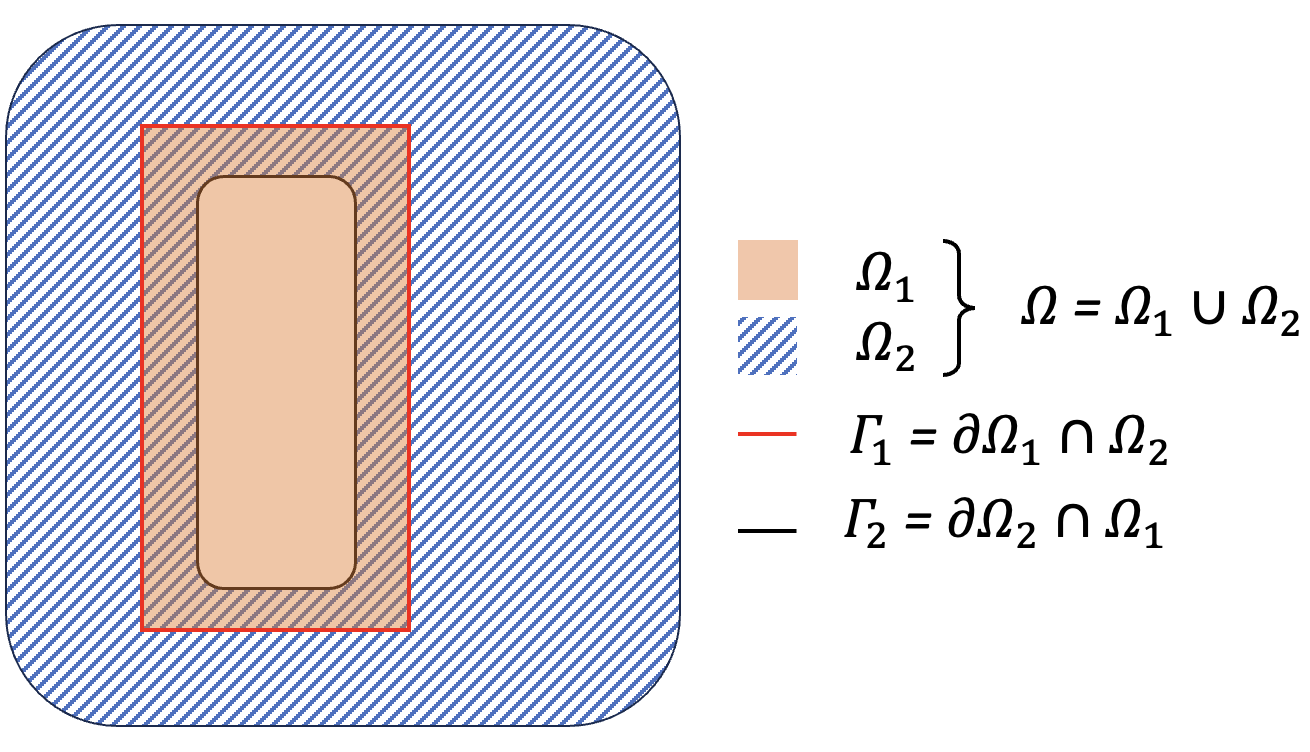
\includegraphics[angle=0,width=0.9\textwidth]{fig/overset-diagram.png}
  \caption{A graphical representation of the overset meshes.}
  \label{fig:overset-diagram}
\end{figure}
the PDE defined on $\Omega$ evolves into two subproblems
\begin{align}
  % governing equation
  \mathcal{L}(\bm{u}_1) &= \bm{f} \quad \text{in} \quad \Omega_1 \\
  \mathcal{L}(\bm{u}_2) &= \bm{f} \quad \text{in} \quad \Omega_2\\
  % boundary conditions
  \bm{u}_1 &= \bm{u}_D \quad \text{on} \quad \partial \Omega_1 \cap \partial \Omega\label{eq:gov-dirichlet-bc1} \\
  \bm{u}_2 &= \bm{u}_D \quad \text{on} \quad \partial \Omega_2 \cap \partial \Omega\label{eq:gov-dirichlet-bc2}
\end{align}
On the newly exposed boundaries due to the domain decomposition, we enforce the solution continuity as Dirichlet boundary condition,
\begin{align}
  \bm{u}_1 = \bm{u}_2 \quad \text{on} \quad \partial \Omega_1 \backslash \partial \Omega\\
  \bm{u}_2 = \bm{u}_1 \quad \text{on} \quad \partial \Omega_2 \backslash \partial \Omega
\end{align}
Conventional solution approaches often rely on original or variants of SAM, which can be summarized below:
% Algorithm of SAM
\begin{enumerate}\label{alg:sam}
  \item Initialize $\bm{u}_1^0$ and $\bm{u}_2^0$.
  \item Solve $\mathcal{L}(\bm{u}_1^{n+1}) = \bm{f}$ in $\Omega_1$ with $\bm{u}_2^n$ as the boundary condition.
  \item Solve $\mathcal{L}(\bm{u}_2^{n+1}) = \bm{f}$ in $\Omega_2$ with $\bm{u}_1^{n+1}$ as the boundary condition.
  \item Repeat Step 2 and 3 until convergence.
\end{enumerate}
Several drawbacks are noticeable for SAM as a domain decomposition solver for nonlinear problems in overset. 
The convergence is conditionally dependent on the overlapping ratio of the overset meshes, completeness of Jacobian matrices, mesh resolution, and PDE operators.
%Even if SAM converges, the convergence rate can be slow, leading to a large number of iterations. \\
When all the conditions for converging are satisfied, the convergence rate could be considerably slow due to a large number of iterations.
In order to address these issues in SAM, we propose a monolithic overset framework.\\
We reserve superscript $h$ for the discrete counterparts. For example, the solution field $\bm{u}_i$ is discretized on the mesh $\Omega_i^h$ as
\begin{align}
  \bm{u}^h_i\in\mathbb{V}^h_i\subset \{\bm{y}\in H^1(\Omega_i^h): \bm{y}|_{\partial\Omega_i\cap\partial\Omega}=\bm{u}_D\}
\end{align}
The testing function space is defined in a similar way
\begin{align}
\bm{w}_i^h\in\mathbb{W}_i^h \subset\{\bm{y}\in H^1(\Omega_i^h): \bm{y}|_{\partial\Omega_i\cap\partial\Omega}=\bm{0}\}
\end{align}
Then, the weak form and the resulting algebraic equations of the governing equations read
\begin{align}%\label{eq:gov-weak-form}
  %
  \mathcal{B}(\bm{w}^h_i, \bm{u}^h_i) - \left(\bm{w}^h_i, \bm{f}\right)
  &=0\quad\forall \bm{w}^h_i\in \mathbb{W}_i
  &\Rightarrow\bm{F}_i(\bm{U}_{i}) = \bm{0}\label{eq:gov-weak-form-pde}\\
  %
  \bm{u}^h_i - \bm{u}^h_{3-i}
  &= \bm{0}\quad\text{on}\quad {\partial \Omega_i\backslash\partial \Omega}
  &\Rightarrow\bm{G}_i(\bm{U}_{i}, \bm{U}_{3-i}) = \bm{0}\label{eq:gov-weak-form-alternative}
\end{align}
In the above equations given $i=1, 2$, 
$\mathcal{B}$ is the weak form operator of the PDE operator $\mathcal{L}$, 
$\bm{U}_{i}$ is a vector of all the degrees of freedoms (DoFs) in $\bm{u}^h_i$, 
$\bm{F}_i$ is the algebraic function derived from Eq.~\ref{eq:gov-weak-form-pde}, 
and $\bm{G}_i$ is the function enforcing the solution continuity. 
We call the residual derived from Eq.~\ref{eq:gov-weak-form-alternative} and Eq.~\ref{eq:gov-weak-form-alternative} as PDE and alternative residual, respectively.
Without further specification, the problem discussed below is scalar-valued for simplicity.\\
Let $\overline{M}_i\,(<\infty)$ denote the number of DoFs in 
$\mathbb{V}_i$, of which ${M}^{\Gamma}_{i}$ are on the newly exposed boundaries and the rest 
$M_{i}=\overline{M}_i-M^{\Gamma}_{i}$ are from either the internal nodes or imposition of 
Dirichlet boundary conditions in Eqs.~\ref{eq:gov-dirichlet-bc1} and~\ref{eq:gov-dirichlet-bc2}. Without loss of generality, we assume the DoFs on 
$\partial\Omega_i\backslash\partial\Omega$ always have larger indices than the others. Therefore, $\bm{G}_i$ can be written as
\begin{align}
  \bm{G}_i(\bm{U}_{i}, \bm{U}_{3-i}) = \bm{S}_i\bm{U}_{i} - {\Pi}_i\bm{U}_{3-i}
\end{align}
$\bm{S}_i$ and ${\Pi}_i$ in the above equation are the selection and projection matrices, respectively
\begin{align}
  [\bm{S}_i]_{M^\Gamma_i\times \overline{M}_i}&=
  \begin{bmatrix}
    \bm{O}_{M^\Gamma_i\times M_i} & \bm{I}_{ M^\Gamma_i \times M^\Gamma_i}
  \end{bmatrix}\\
  [{\Pi}_i]_{M^\Gamma_i \times \overline{M}_{3-i}}&=
  \sum_{j=1}^{M^\Gamma_i}\bm{e}^\Gamma_{j} \bm{p}_{i,j}^T
\end{align}
where $\bm{e}^\Gamma_{j}$ is a vector with the $(j+M_i)$-th entry being 1 and the rest being 0, $\bm{p}_{i,j}$ is a vector such that 
\begin{align}
  \bm{u}^h_{3-i}({\bm{x}_{i,j+M_i}})=\bm{p}_{i,j}^T \bm{U}_{3-i}
\end{align}
with $\bm{x}_{i,j+M_i}$ denoting the coordinate 
of the $j+M_i$-th node on $\Omega_i^h$. 
The construction of $\bm{p}_{i,j}$ contains two steps: locating the element $\Omega_{3-i}^h$ that contains $\bm{x}_{i,j+M_i}$ before
evaluating the shape function values of the node with respect to the element.\\
Define $\varphi(\bm{x}, \Omega_i^h)$ as the index of an element in $\Omega_i^h$ that contains $\bm{x}$, 
$\bm{R}_{i,j}$ as the algebraic restriction of $\bm{U}_i$ to the DoFs associated with the $j$-the element of $\Omega_i^h$, 
and $\bm{W}_{i,j}$ as the shape function values of the node with respect to the $j$-the element.
Then $\bm{p}_{i,j}$ can be further decomposed into
\begin{align}
  \bm{p}_{i,j}^T = \bm{W}_{3-i,\phi}^T\bm{R}_{3-i,\phi}
\end{align}
where $\phi=\varphi(\bm{x}_{i,j}, \Omega_{3-i}^h)$.
Therefore, $\bm{\Pi}_{i}$ reads
\begin{align}
  \bm{\Pi}_i=\sum_{j=1}^{M^\Gamma_i}\bm{e}^\Gamma_{j} \bm{W}_{(3-i),\phi}^T\bm{R}_{(3-i),\phi}
\end{align}
The monolithic overset framework is to solve the nonlinear problem as a whole system using Newton's method, so the following 
notations become necessary,
\begin{align}
  \bm{U} =
  \begin{bmatrix}
    \bm{U}_{1}\\
    \bm{U}_{2}
  \end{bmatrix}
  \quad\text{and}\quad
  \bm{F} =
  \begin{bmatrix}
    \bm{F}_1 & \bm{0}\\
    \multicolumn{2}{c}{\bm{G}_1}\\
    \bm{0} & \bm{F}_2\\
    \multicolumn{2}{c}{\bm{G}_2}
  \end{bmatrix}
  =
  \begin{bmatrix}
    \bm{F}_1 & \bm{0}\\
    \bm{S}_1 & -\Pi_1\\
    \bm{0} & \bm{F}_2\\
    -\Pi_2 & \bm{S}_2
  \end{bmatrix}
\end{align}
The Jacobian matrix
of the nonlinear system reads
\begin{align}
  \bm{J}
  =\frac{\partial \bm{F}\left(\bm{U}\right)}{\partial \bm{U}}
  =\left[
    \begin{array}{c;{2pt/2pt}c}
      \begin{matrix}
        \multicolumn{2}{c}{{\partial \bm{F}_1}/{\partial \bm{U}_{1}}} \\
        \bm{0} & \bm{I}
      \end{matrix}
      &
      \begin{matrix}
        \bm{0}\\
        -\Pi_1
      \end{matrix}
      \\ \hdashline[2pt/2pt]
      \begin{matrix}
        \bm{0} \\ 
        -\Pi_2
      \end{matrix}
      &
      \begin{matrix}
        \multicolumn{2}{c}{{\partial \bm{F}_2}/{\partial \bm{U}_{2}}} \\
        \bm{0} & \bm{I}
      \end{matrix}
    \end{array}
  \right]
\end{align}
In contrast to SAM~\ref{alg:sam}, the algorithm of the monolithic overset 
framework can be summarized as follows:
\begin{enumerate}
  \item Initialize $\bm{U}^{[0]}$.
  \item Solve $\bm{J}|_{\bm{U}=\bm{U}^{[n]}}\delta\bm{U} = -\bm{F}(\bm{U}^{[n]})$.
  \item Update $\bm{U}^{[n+1]} = \bm{U}^{[n]} + \delta\bm{U}$.
  \item Repeat Step 2 and 3 until convergence.
\end{enumerate}
The proposed monolithic approach has better convergence and robustness
than its iterative counterpart. It is further discussed in the following sections.
\subsection{Parallelization}\label{sec:parallelization}
The computational cost of overset problems could be high, especially for large-scale problems.
Therefore, it is crucial to accelerate the computation by parallelization. This section focuses on the
parallelized layout of residual vectors and  Jacobian matrices.\\
Element-wise mesh partitioning is adopted using METIS~\cite{karypis1998fast} to achieve load balance. In
this way, the mesh is partitioned into subdomains, and each subdomain is assigned to a processor.
The elements are exclusively owned by the processor that contains the element, leading to the shared DoFs
on the subdomain boundaries.\\
For the residual vector, the parallelization is straightforward. Globally, the assembly of the residual 
vector is to add the element-wise residual vector $\bm{b}_{i,e}$, from $e$-th element of $\Omega_i^h$, 
to the global residual vector,
\begin{align}
  \bm{b} =
  \begin{bmatrix}
    \bm{b}_1\\
    \bm{b}_2
  \end{bmatrix}
\end{align}
and 
\begin{align}
  \bm{b}_i=\sum_{e=1}^{M^E_i}\bm{R}^T_{i,e}\bm{b}_{i,e}
\end{align}
The transpose $\bm{R}^T_{i,e}$ is an extension-by-zero matrix, which extends the element-wise residual vector
to a length $\overline{M}_i$ vector by padding with zero.\\
We partition $\Omega_i^h$'s element indices $1, 2, ..., M^E_i$ ($M^E_i<\infty$ is the number of elements in $\Omega_i^h$)
into $M_p$ disjoint subsets
$\mathcal{E}_{i,j} \in \{1, 2, ..., M^E_i\}, \quad j=1, 2, ..., M_p$.
The $j$-th processor owns the elements in $\mathcal{E}_{i,j}$, and the local residual vector is
\begin{align}
  \bm{b}^{(p)}_i = 
    \sum_{e\in\mathcal{E}_{i,p}}\overline{\bm{R}}^T_{i,e}\bm{b}_{i,e}
\end{align}
where $\overline{\bm{R}}_{i,e}$ is similar to $\bm{R}_{i,e}$, but only extracts the DoFs from 
processor-local residual vectors and the global assembly is 
\begin{align}
  \bm{b}_i = \sum_{p=1}^{M_p} {\tilde{\bm{R}}}^T_{i,p}\bm{b}^{(p)}\label{eq:vector-assembly}
\end{align}
with $\tilde{\bm{R}}$ being the restriction of the global residual vector to the local one.
Fig.~\ref{fig:restriction} presents the relationship among $\bm{R}_{i,e}$, $\overline{\bm{R}}_{i,e}$, and $\tilde{\bm{R}}_{i,p}$\\
\begin{figure}[!htbp]
  \centering
  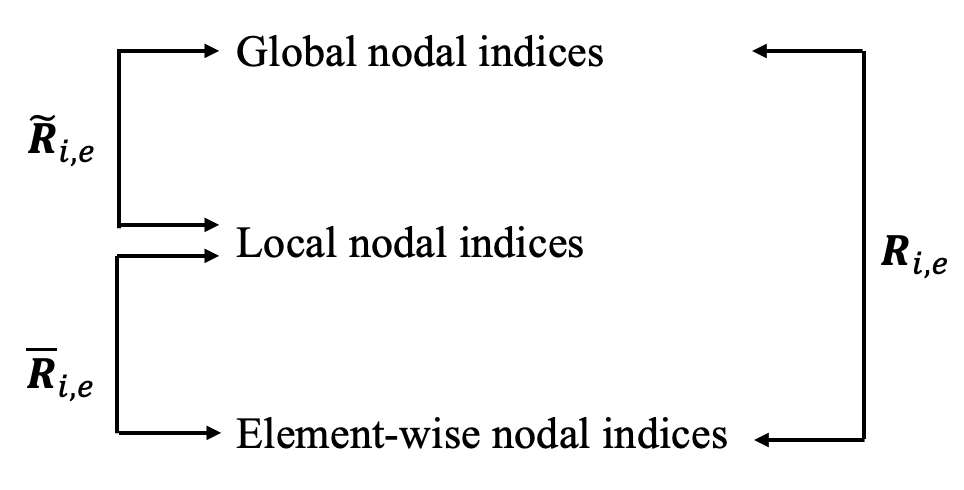
\includegraphics[angle=0,width=0.8\textwidth]{fig/algebraic-restriction.png}
  \caption{The relationship among $\bm{R}_{i,e}$, $\overline{\bm{R}}_{i,e}$, and $\tilde{\bm{R}}_{i,p}$.}
  \label{fig:restriction}
\end{figure}
It is noticeable that shared DoFs exist on the subdomain boundaries. A popular approach 
is to use ghost DoFs. 
To be more specific, let us fix one DoF, and among all the processors that contain the DoF, one is chosen as the owner processor.
For the other processors, the DoF is called a ghost DoF, and the values of the DoF are communicated to the owner processor for the assembly.
After that, the owner processor broadcasts its value to all the processors that contain the DoF.

The Jacobian matrix assembly follows
\begin{align}
  \bm{K}_i
  :=\frac{\partial\bm{b}_i}{\partial \bm{U}_{i}} 
  =\sum_{e=1}^{M^E_i}\bm{R}^T_{i,e}\frac{\partial\bm{b}_{i,e}}{\partial \bm{U}_{i}}
  =\sum_{e=1}^{M^E_i}\bm{R}^T_{i,e}\frac{\partial\bm{b}_{i,e}}{\partial \bm{U}_{i}^e}\bm{R}_{i,e}
\end{align}
where $\bm{U}_{i}^e$ is the element-wise DoFs of $\bm{U}_{i}$. Similarly, the matrix of each processor follows
\begin{align}
  \bm{K}^{(p)}_i &= \sum_{e\in\mathcal{E}_{i,p}}\overline{\bm{R}}^T_{i,e}\frac{\partial\bm{b}_{i,e}}{\partial \bm{U}_{i}^e}\overline{\bm{R}}_{i,e}\\
  \bm{K}_i &= \sum_{p=1}^{M_p}\left[\tilde{\bm{R}}^T_{i,p}\bm{K}^{(p)}_i \tilde{\bm{R}}_{i,p}\right]
\end{align}
The parallelization of the Jacobian matrix requires the data synchronization of the matrix entries, of which either the row indices or column indices are shared by multiple processors, leading to more complicated communication patterns. 
To avoid the heavy communication overhead, we adopt a zero-communication matrix layout since the matrix-vector multiplication is a composition of the processor-local submatrix-vector multiplications.
Specifically,
\begin{align}
  \nonumber \bm{K}_i \bm{b}_i &= \left[\sum_{p=1}^{M_p} \tilde{\bm{R}}^{T}_{i,p}\bm{K}^{(p)}_i \tilde{\bm{R}}_{i,p}\right]\bm{b}_i \\
                              &= \sum_{p=1}^{M_p}\tilde{\bm{R}}^{T}_{i,p} \left[\bm{K}^{(p)}_i \tilde{\bm{R}}_{i,p}\bm{b}_i\right]
\end{align}
where $\bm{K}^{(p)}_i \tilde{\bm{R}}_{i,p}\bm{b}_i$ can be computed locally on the $p$-th processor. 
The remaining operation is the same as the residual vector assembly described in Eq.~\ref{eq:vector-assembly}.
It is worth noticing that the above assembly fashion is designed for the vector components and the submatrices derived from the PDE residual defined in Eq.~\ref{eq:gov-weak-form-pde}. 
The extra vector entries and Jacobian subblocks from the alternative residual of Eq.~\ref{eq:gov-weak-form-alternative} need a compatible assembly fashion. See the following section for more details.
\subsection{Composited and Matrix-free Jacobian Matrix}
This section's concentration is the Jacobian matrix implementation, especially for the newly added submatrices $\Pi_i$ induced by the monolithic overset framework.
Despite the given explicit expression, many difficulties exist in implementing it.
%First, both $\partial \bm{F}_i/\partial \bm{U}_{i}$ and $\Pi_i$ are sparse matrices, while they follow different sparsity patterns.
%The former sparsity pattern relies on the connectivity of the nodal graph generated by the mesh. The latter one is the off-diagonal non-square 
%block matrix, representing the relationship between two independent meshes without any inter-mesh connectivity, which can not be precomputed 
%until collision detection is performed. Second, the ghost DoFs ensure the vector entries have at least one copy if needed by local patches of the 
%Jacobian matrix $\bm{K}_i^{(e)}$ in matrix-vector multiplication . However, the ghost DoFs are insufficient since the multiplication needs
%the vector entries from another processor, another mesh, which is unavailable in the ghost DoFs. Third, the sparsity pattern of $\Pi_i$ 
%requires dynamic allocation due to the relative motion of the meshes. For example, a node on the mesh $\Omega_1$ may leave the element of 
%$\Omega_2$ in the previous step and enter another element, even a subdomain belonging to another processor, during the mesh rotation. Therefore,
%each time step needs to update the sparsity pattern of $\Pi_i$.
First, the sources of sparsity patterns are incompatible between $\partial \bm{F}_i/\partial \bm{U}_{i}$ and $\partial \bm{G}_i/\partial \bm{U}$.
The sparsity pattern generation for compressed sparse row format relies on the nodal connectivity graph of meshes.
It works well with the submatrices $\partial \bm{F}_i/\partial \bm{U}_{i}$, but not $\partial \bm{G}_i /\partial \bm{U}$,
whose sparsity pattern relies on the mapping between the nodes of $\Omega_i^h$ and the elements of $\Omega_{3-i}^h$.
Second, the mapping between the nodes and the elements is dynamically changing due to the relative motion of the meshes.
Therefore, the precomputation of the sparsity pattern is impossible, and dynamic allocation is required every time step to update the sparsity pattern despite the high temporal cost.
The above difficulties make the direct implementation of the Jacobian extraordinarily complicated. \\
We propose a composited and partially matrix-free Jacobian assembly to address the above difficulties.
Specifically, the Jacobian matrix $\bm{J}$ is a composition of submatrices, which needs dealing with separately.
Submatrices $\partial \bm{F}_i/\partial \bm{U}_{i}$ follow the procedure of the conventional Jacobian assembly in Section~\ref{sec:parallelization}. 
The abovementioned issues lead to a matrix-free $\Pi_i$, which needs an algorithm to evaluate the matrix-vector multiplication vector rather than a physical copy of matrix entries on memory. 
The resulting vector computation is
\begin{align}
  \frac{\partial \bm{G}_i}{\partial \bm{U}}
  \begin{bmatrix}
    \bm{X}\\
    \bm{Y}
  \end{bmatrix}
  =
  \begin{bmatrix}
    \bm{0} & \bm{I}
  \end{bmatrix}
  \bm{X} - \Pi_i\bm{Y}
\end{align}
where two terms are evaluated separately before a value collection of $\Pi_i\bm{Y}$ and subtraction.
The first term is equivalent to the extraction of the last $M^\Gamma_i$ DoFs from $\bm{X}$, and the second term interpolation of $\bm{Y}$ onto the specific nodes
using the corresponding mesh.
\begin{figure}
  \center
  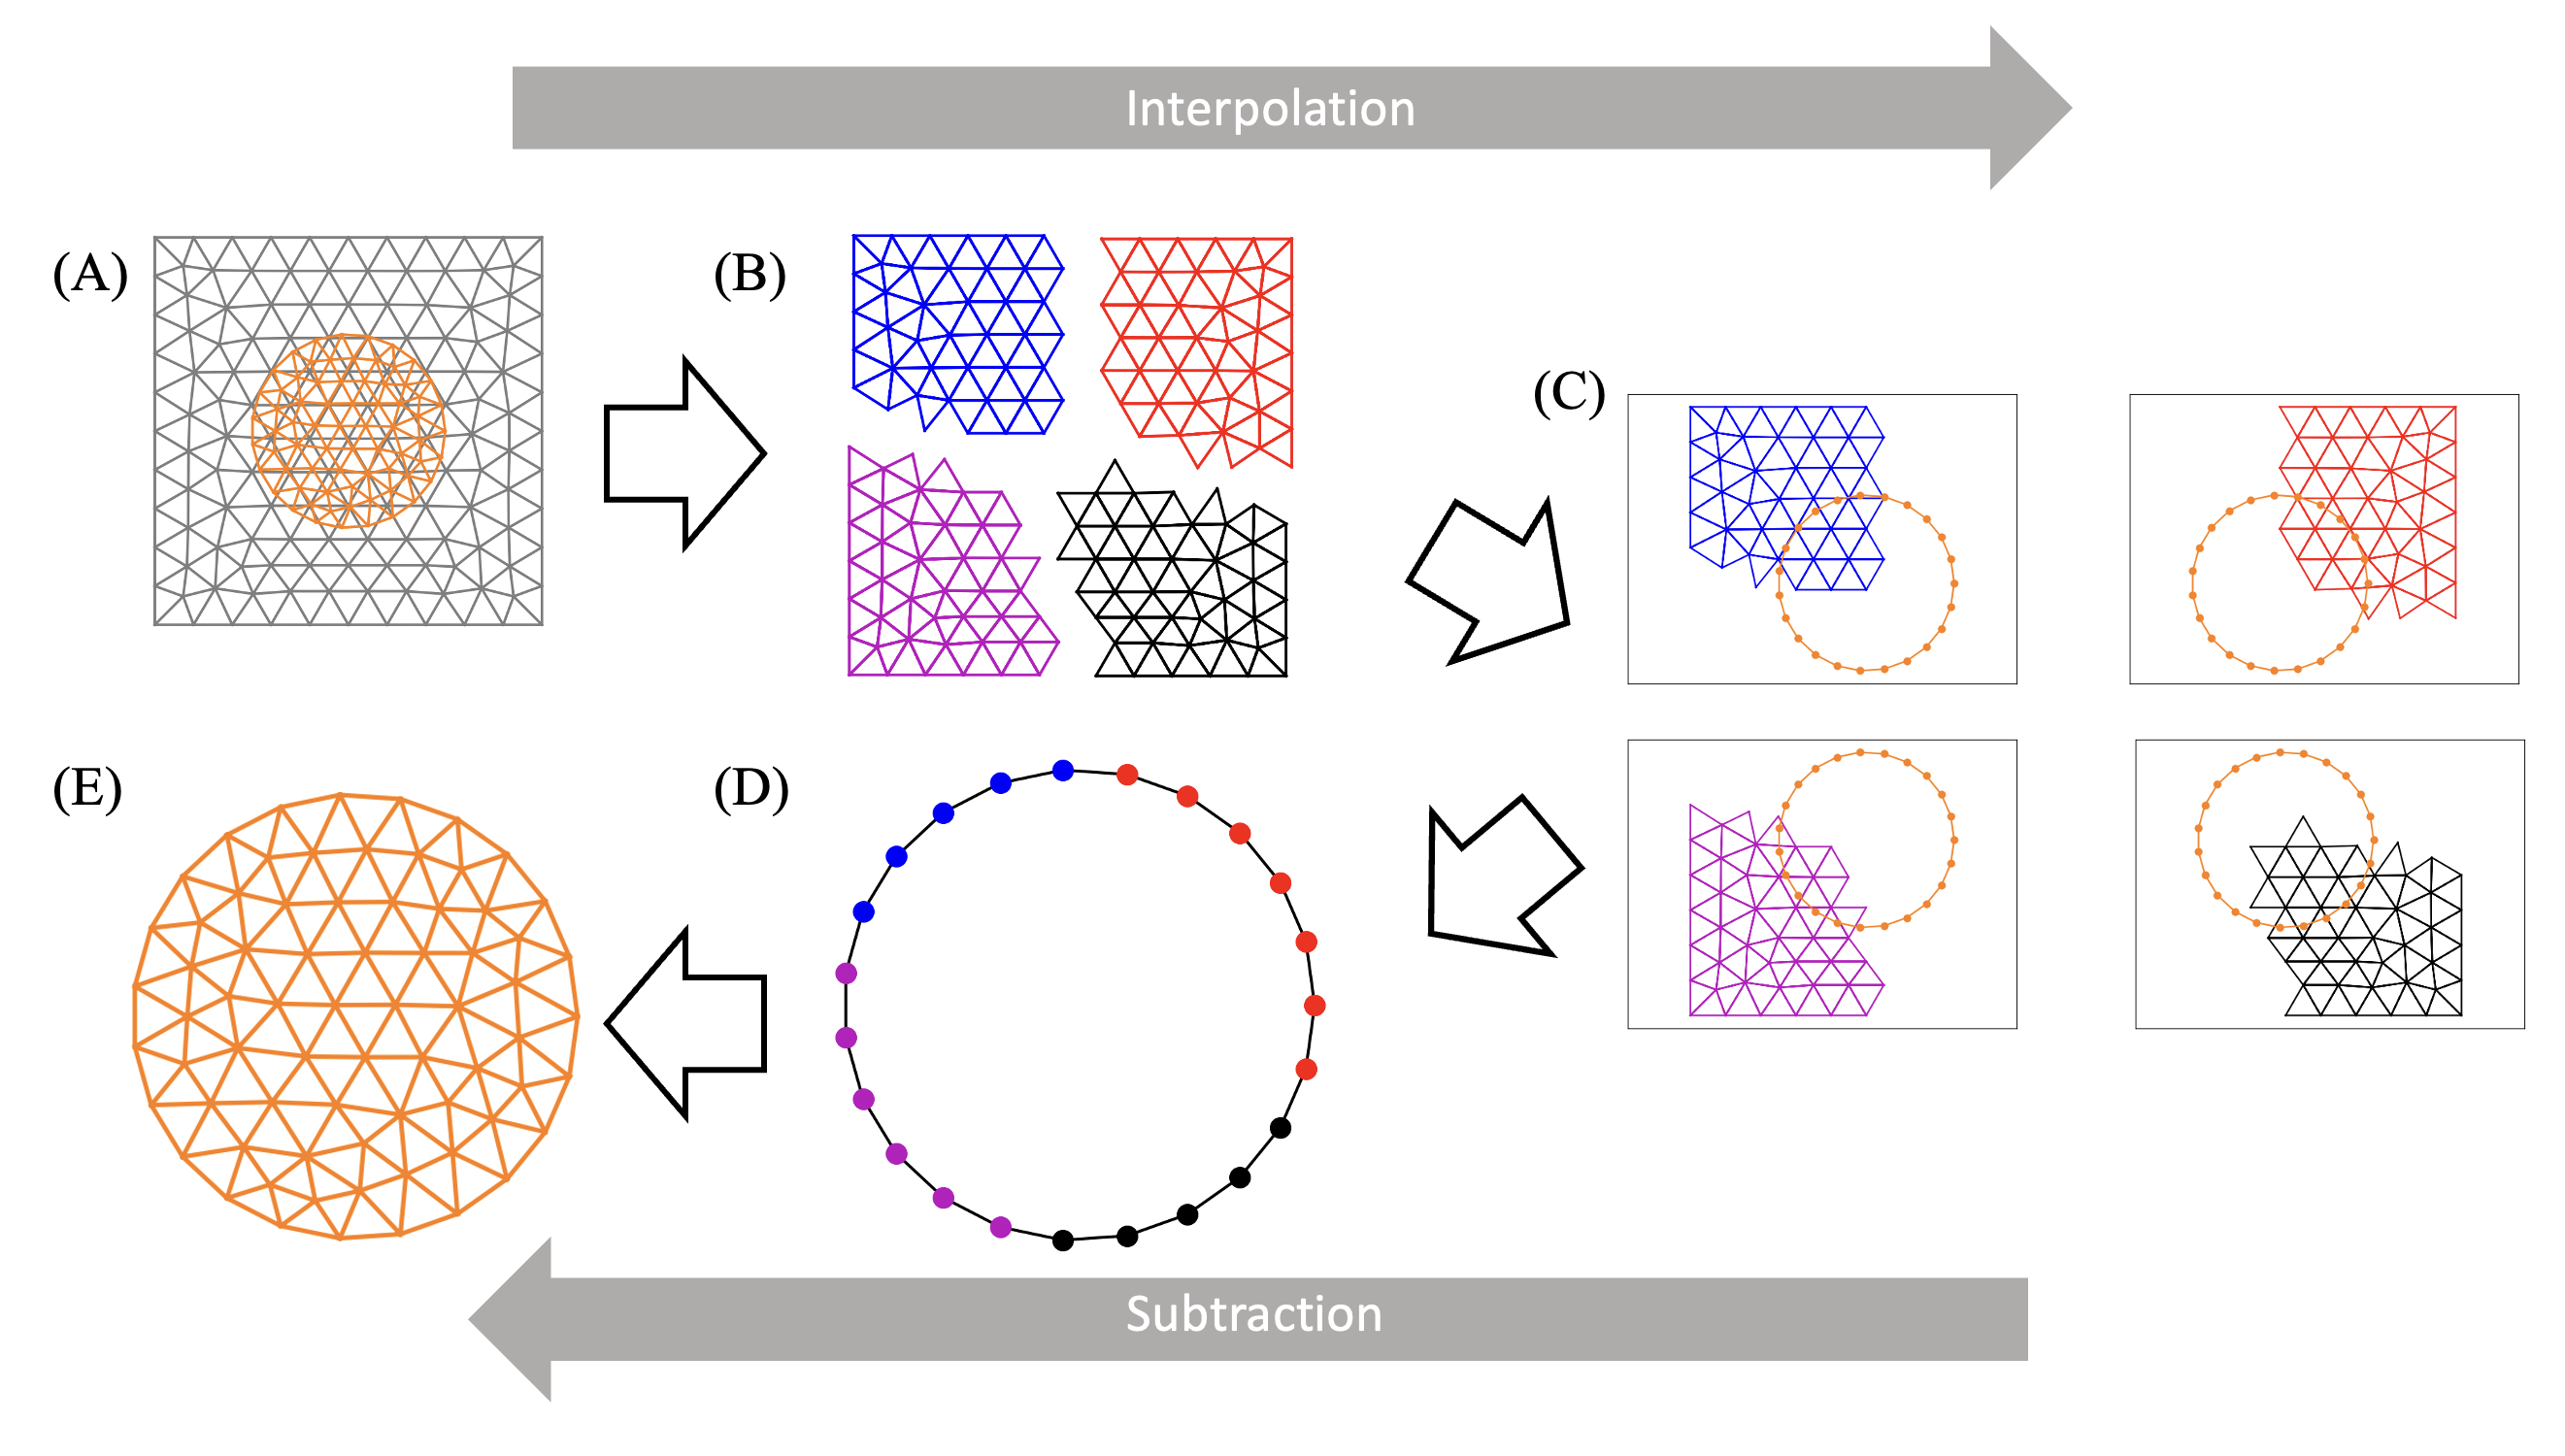
\includegraphics[width=1.0\textwidth]{fig/overset-residual-evaluation.png}
  \caption{The evaluation of the alternating residual and the multiplication of the matrix-free Jacobian blocks.}
  \label{fig:overset-residual-evaluation}
\end{figure}
The details of the computation include the following steps (see Fig.~\ref{fig:overset-residual-evaluation}):
\begin{enumerate}
  \item Load the overset meshes and the solution fields. A complete surface mesh of the newly exposed boundaries is also loaded for each processor.
  \item Partition the meshes using METIS~\cite{karypis1998fast}.
  \item Interpolate the values onto the surface mesh nodes as long as a local element encloses the nodes.
  \item Synchronize the values of the surface mesh nodes among processors.
  \item Subtract the values of the surface mesh nodes from the corresponding nodes of the solution fields.
\end{enumerate}
\subsection{Octree-based Collision Detection}\label{sec:octree}
In Section~\ref{sec:monolithic-overset-framework}, a key component is the calculation of the element indices containing a specific coordinate 
$\phi_i,j$ which relies on collision detection. However, the naive approach is computationally expensive, resulting in a complexity
~$\mathcal{O}(M^E_i)$, especially for large-scale problems. Therefore, we utilize the octree data structure to accelerate the collision 
detection, which satisfies $\mathcal{O}(log M^E_i)$.\\
\begin{figure}[!htpb]
	\centering
	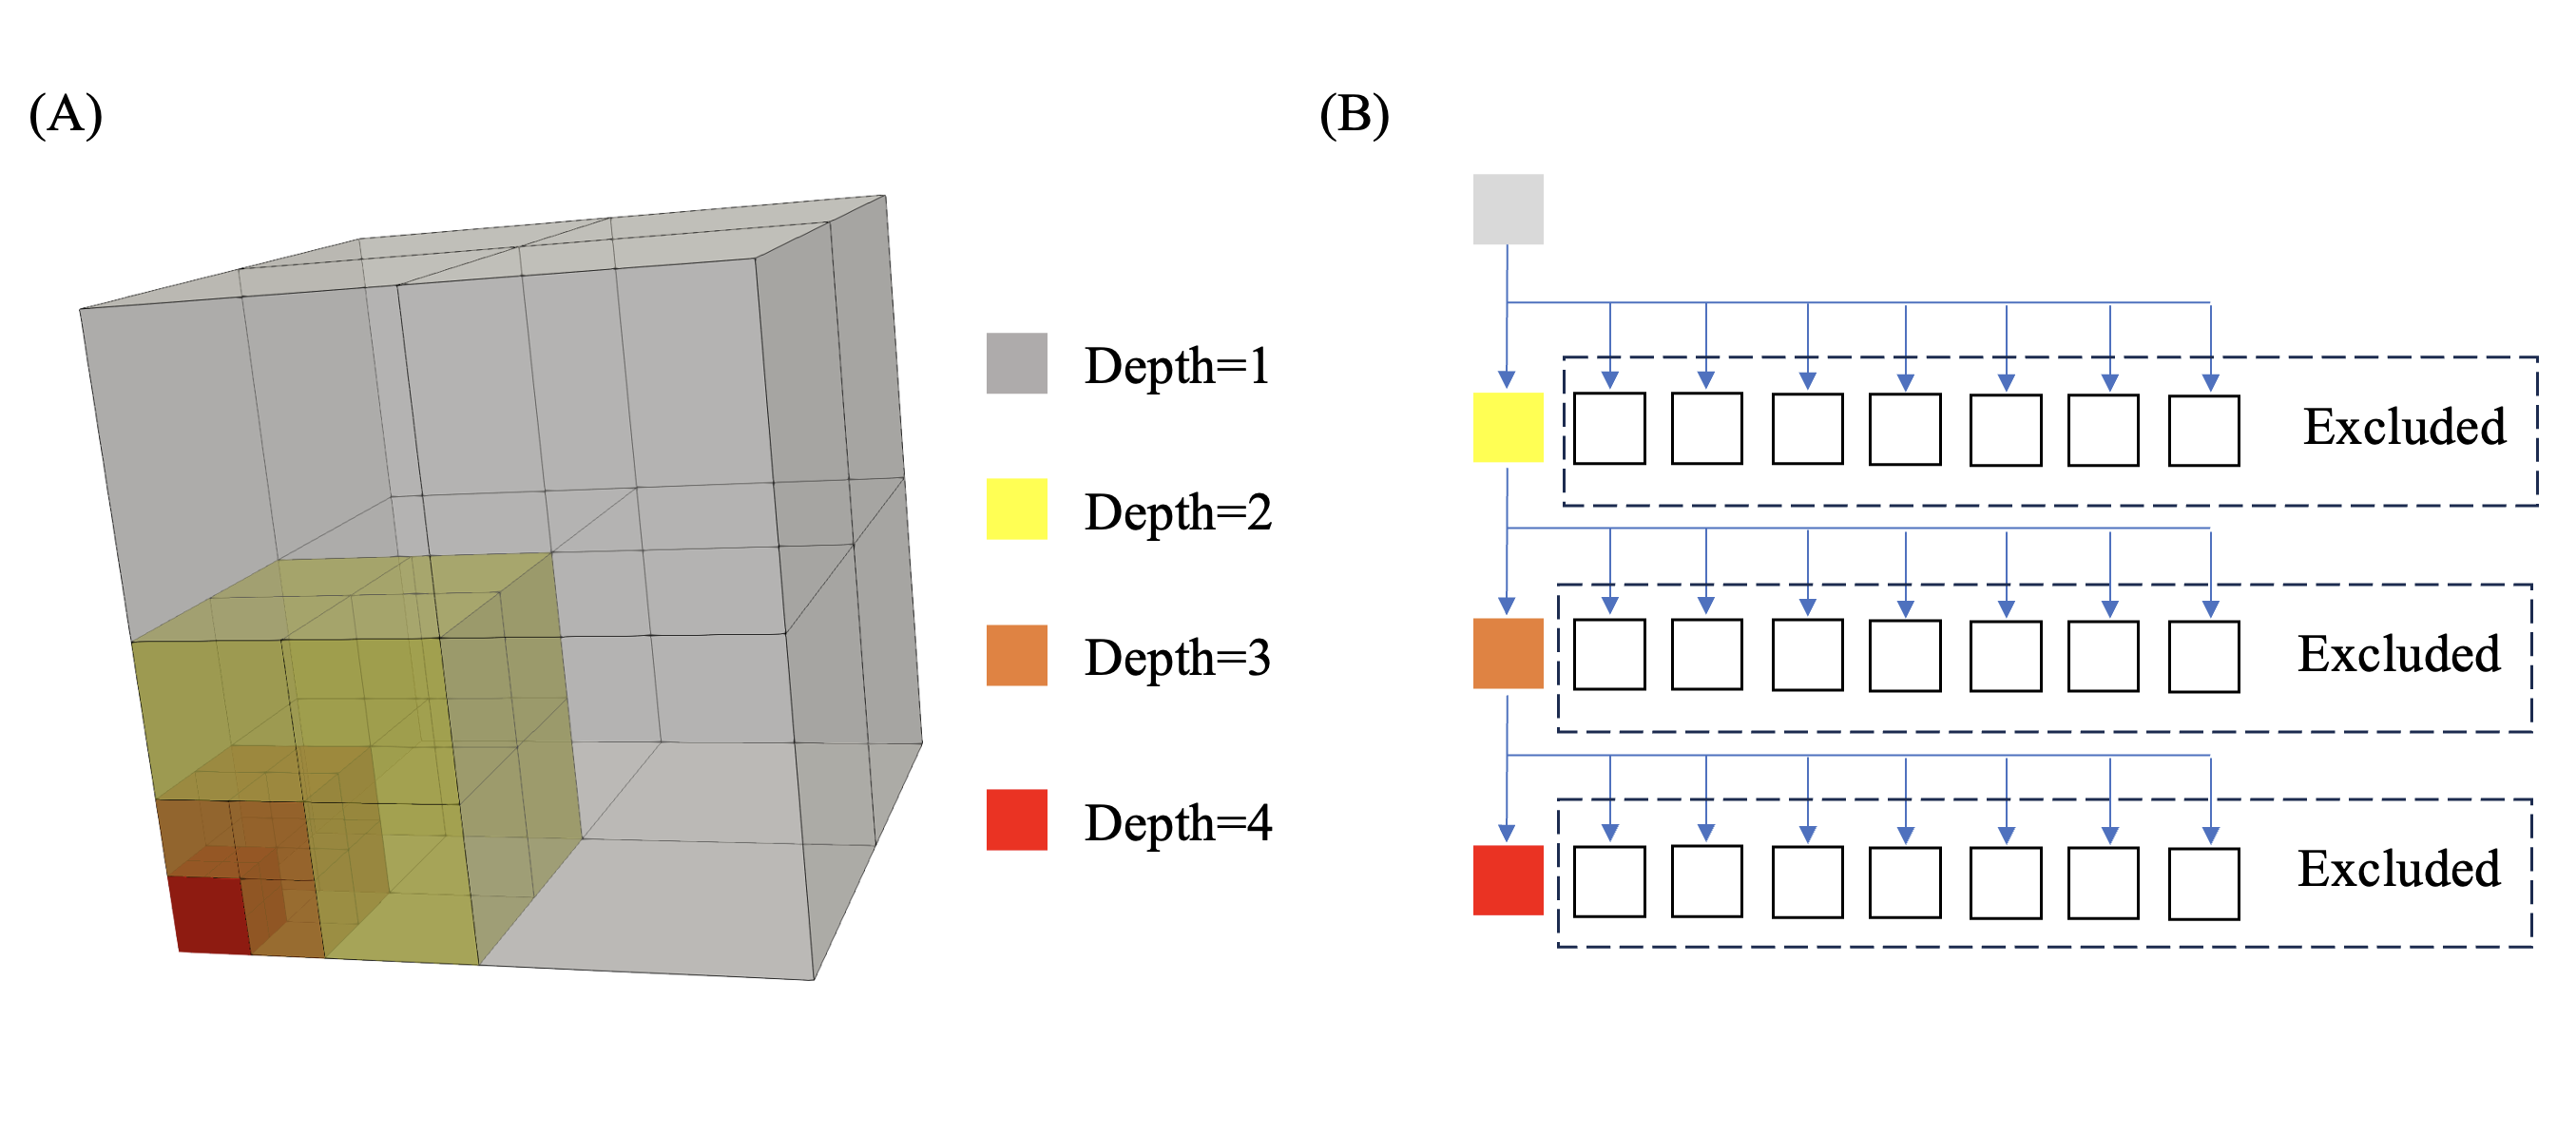
\includegraphics[angle=0,width=1.\textwidth]{fig/octree-diagram.png}
	\caption{Octree speeds up collision detection. (A) The domain is recursively subdivided into eight octants, the maximal depth of which
    is 4. (B) When octree is used for collision detection between nodes and elements, the octants that do not contain any nodes can be 
    excluded from the collision detection.}
	\label{fig:octree}
\end{figure}
The octree data structure is a tree in which each internal node has exactly eight children. The octree is constructed by
recursively subdividing the domain into eight octants, and each octant is further subdivided into eight octants until the number of elements
in the octant is less than a threshold or a maximal depth is reached. A bounding box is constructed for every single octant, representing the
spatial extent of the octant. The bounding box of an octant is the smallest axis-aligned bounding box that contains all the elements in the
octant. An octree is constructed for each mesh and updated in each time step. The collision detection is performed by traversing the octree
from the root node in a depth-first way. This method has been validated in~\cite{Xu16ig, zhu2020immersogeometric, zhao2022enriched} for compatibility with the FEM framework and efficiency compared with
the conventional searching algorithm. \\
When working with ALE, octree needs a stepwise update. The algorithm is carefully
implemented to ensure efficiency in both construction and searching.
\subsection{Formulation of incompressible flow}
The ALE~\cite{bazilevs2012ale} form of the multiscale formulation for incompressible flow~\cite{Bazilevs07b} reads: find $\{{\bm{u}}^h, p^h\}\in\mathbb{V}^h$, such that $\forall\{\bm{w}^h, q^h\}\in\mathbb{W}^h$,
\begin{align}
  B_M\left(\bm{w}^h, \{\bm{u}^h, p^h\}\right) + B_C\left(q^h, \{\bm{u}^h, p^h\}\right) = 0
\end{align}
\begin{align}
  % Momentum
  % Momentum: Coarse scale
  \nonumber B_M\left(\bm{w}^h, \{\bm{u}^h, p^h\}\right)
  =&\left(\bm{w}^h, \rho(\dot{\bm{u}}^h+(\bm{u}^h-\hat{\bm{u}})\cdot\nabla\bm{u}^h-\bm{b})\right)
  -\left(p^h, \nabla\cdot\bm{w}^h\right)\\
  \nonumber +&\left(\nabla\bm{w}^h, \mu\nabla\bm{u}^h\right)
  + \left( (\nabla\bm{w}^h)^T, \mu\nabla\bm{u}^h\right)  \\
  % Momentum: Fine-scale
  \nonumber +&\sum_e \left(\rho\tau_M (\bm{u}^h-\hat{\bm{u}})\cdot\nabla \bm{w}^h, \bm{r}^M\right)_{\Omega_e}
  +\sum_e\left(\nabla\cdot\bm{w}^h, \rho \tau_C \nabla\cdot\bm{u}^h\right)_{\Omega_e}\\
  \nonumber -&\sum_e\left(\bm{w}^h, \rho\tau_M\bm{r}^M\cdot\nabla\bm{u}^h\right)_{\Omega_e}
  -\sum_e\left(\rho\tau_M^2\nabla\bm{w}^h,\bm{r}^M\otimes\bm{r}^M \right)_{\Omega_e}\\
  +&\sum_e\left(\rho\overline{\tau}\tau_M^2 \bm{r}^M\cdot\nabla\bm{w}^h, \bm{r}^M\cdot\nabla\bm{u}^h\right)_{\Omega_e}\\
  % Continuity
  % Continuity: Coarse scale
  B_C\left(q^h, \{\bm{u}^h, p^h\}\right)=&\left(q^h, \nabla\cdot\bm{u}^h\right)
  % Continuity: Fine-scale
  +\sum_e\left(\nabla q^h,\tau_M\bm{r}^M\right)_{\Omega_e}
\end{align}
where $\rho$ is the density of the fluid, $\bm{u}^h$ is the velocity field, $\hat{\bm{u}}$ is the mesh motion velocity, $p^h$ is the pressure field,
$\bm{b}$ is the body force, $\mu$ is the dynamic viscosity. Stabilization parameters $\tau_M$, $\tau_C$, and $\overline{\tau}$ are defined in~\cite{Brooks82a, Tezduyar91c, hughes1989new}, 
and validated or verified in~\cite{du2023modeling, zhao2023computational, zhao2022enriched, zhu2021mixed, zhao2020variational,Kamensky15ch, Kamensky2017, hsu2012wind, Akkerman11a, Akkerman11b}.
\begin{align}
  \tau_M&=\left(\frac{4}{\Delta t^2}+(\bm{u}^h-\hat{\bm{u}})\cdot\bm{G}\cdot(\bm{u}^h-\hat{\bm{u}})+C_I(\frac{\mu}{\rho})^2 \bm{G}:\bm{G}\right)^{-1/2}\\
  \tau_C&=\frac{\left((\bm{u}^h-\hat{\bm{u}})\cdot\bm{G}\cdot(\bm{u}^h-\hat{\bm{u}})+C_I(\frac{\mu}{\rho})^2 \bm{G}:\bm{G}\right)^{1/2}}{tr(\bm{G})}\\
  \overline{\tau}&=\left(\tau_M^2\bm{r}\cdot\bm{G}\cdot\bm{r}\right)^{-1/2}
\end{align}
where $\Delta t$ is the time step length, $\bm{G}$ is the element-wise metric tensor, and $C_I$ is typically equal to 4~\cite{Bazilevs07b,Tezduyar00a}.
Besides, $\bm{r}^M$ is the momentum residual, which is defined as
\begin{align}
  \bm{r}^M = \rho(\dot{\bm{u}}^h+(\bm{u}^h-\hat{\bm{u}})\cdot\nabla\bm{u}^h-\bm{b}) + \nabla p^h - \mu\nabla^2\bm{u}^h
\end{align}
%\begin{align}
%  \bm{u}^h = \bm{u}^h_D \quad \text{on} \quad \Gamma_D
%\end{align}
For time integration, we incorporate the generalized-$\alpha$ method~\cite{jansen2000generalized}, 
\begin{align}
  \dot{\bm{u}}^h_{n+\alpha_m} &= \dot{\bm{u}}^h_{n} + \alpha_m (\dot{\bm{u}}^h_{n+1} - \dot{\bm{u}}^h_{n})\\
  \bm{u}^h_{n+\alpha_f} &= \bm{u}^h_{n} + \alpha_f (\bm{u}^h_{n+1} - \bm{u}^h_{n})
\end{align}
and Newmark-$\beta$ scheme~\cite{newmark1959method},
\begin{align}
  \bm{u}_{n+1}^h &= \bm{u}^h_{n} + \Delta t(\gamma \dot{\bm{u}}^h_{n+1} + (1-\gamma)\dot{\bm{u}}^h_{n}) 
\end{align}
where $\alpha_m$, $\alpha_f$, and $\gamma$ are the parameters defined in~\cite{chung1993time}.
In the context of the monolithic overset framework, $\bm{F}_i$ is the residual generated by $B_M$ and $B_C$, and $\bm{U}_{i}$ is the global vector
of DoFs, including nodal velocity and pressure
\begin{align}
  \bm{F}_i = \begin{bmatrix}
    B_M(\{\bm{u}^h_i, p^h_i\}, \bm{w}^h_i)\quad\forall \bm{w}^h_i\text{ such that }\{\bm{w}^h_i, 0\}\in\mathbb{W}^h\\
    B_C(\{\bm{u}^h_i, p^h_i\}, q^h_i)\quad\forall q^h_i\text{ such that }\{\bm{0}, q^h\}\in\mathbb{W}^h
  \end{bmatrix}
\end{align}
and only velocity continuity is enforced across the newly exposed boundaries, namely,
\begin{align}
  \bm{u}_{i,n+1}=\bm{u}_{3-i,n+1} \quad \text{on} \quad \partial\Omega_i\backslash\partial\Omega
\end{align}
Note that under VMS formulation, the velocity consists of coarse and fine scales, $\bm{u}_{i,n+1}=\bm{u}^h_{i,n+1} + \bm{u}^\prime_{i,n+1}$, and 
the fine-scale velocity is zero on the element facets, part of which is the newly exposed boundaries. Therefore, if each 
newly exposed boundary is also on the element facets of the other mesh. The above equation can be further simplified as
\begin{align}
  \bm{u}^h_{i,n+1}=\bm{u}^h_{3-i,n+1} \quad \text{on} \quad \partial\Omega_i\backslash\partial\Omega
\end{align}
Accordingly, the submatrices of the Jacobian matrix evolve into
\begin{align}
  \bm{J}
  =\left[
    \begin{array}{c;{2pt/2pt}c}
      \begin{matrix}
        \multicolumn{2}{c}{{\partial \bm{F}_1}/{\partial \bm{U}^{(1)}}} \\
        \bm{0} & \textcolor{red}{\Delta t\gamma}\bm{I}
      \end{matrix}
      &
      \begin{matrix}
        \bm{0}\\
        -\textcolor{red}{\Delta t\gamma}\Pi_1
      \end{matrix}
      \\ \hdashline[2pt/2pt]
      \begin{matrix}
        \bm{0} \\ 
        -\textcolor{red}{\Delta t\gamma}\Pi_2
      \end{matrix}
      &
      \begin{matrix}
        \multicolumn{2}{c}{{\partial \bm{F}_2}/{\partial \bm{U}^{(2)}}} \\
        \bm{0} & \textcolor{red}{\Delta t\gamma}\bm{I}
      \end{matrix}
    \end{array}
  \right]
\end{align}
Besides, all the simulations are performed with linear elements, lines for one-dimensional space and tetrahedrons for three-dimensional space. The linear system generated from Newton's method is solved
using the block-Jacobian preconditioned generalized minimal residual method (GMRES)~\cite{Saad86a}. 
\section{Numerical Examples}\label{sec:numerical-examples}
\subsection{Burgers' Equation}
We first apply our method to a nonlinear problem, namely, Burgers' equation, which can be treated as a simplification of the Navier-Stokes equation by neglecting the pressure term.
Burgers' equation occurs in many engineering applications involving nonlinear flow behavior, like traffic flow and gas dynamics.
The purpose of this example is to validate the compatibility of the proposed method in nonlinear FEM.
The accuracy of the method is evaluated by comparing the results to the solution from a single-mesh method with sufficient resolution. 
The strong form of the equation within the interval $\Omega=[-1, 1]$ is defined as
\begin{align}\label{eq:burgers-strong}
    \dot{u}+u\frac{\partial u}{\partial x} - \nu \frac{\partial^2 u}{\partial x^2}=0
\end{align}
The initial and boundary conditions are
\begin{align}
    u|_{t=0} & = -sin(\pi x)\\
    u|_{\partial \Omega}&=0
\end{align}
In Eq.~\ref{eq:burgers-strong}, $u:\Omega\times\mathbb{R}^+\rightarrow\mathbb{R}$ is the solution field, and the value of the
diffusion coefficient $\nu=0.01/\pi$.
The weak form is stabilized with SUPG,
\begin{align}
  \nonumber &\left(w^h, \dot{u}^h+u^h\frac{\partial u^h}{\partial x}\right)
  +\left(\frac{\partial w^h}{\partial x},\nu\frac{\partial u^h}{\partial x}\right) \\
  +&\left(\tau_M u^h\frac{\partial w^h}{\partial x}, \dot{u}^h+u^h\frac{\partial u^h}{\partial x}-\nu\frac{\partial^2 u^h}{\partial x^2}\right)= 0
\end{align}

\subsubsection{Convergence}
This part focuses on the convergence behavior in Newton's solver of the proposed method.
We test the solver with different overlapping lengths $\Delta L$, number of elements $M_i^E$, and the time step length $\Delta t$.
The mesh is decomposed into $[-1, \Delta L/2]$ and $[-\Delta L/2, 1]$.
We use the numerical results at $t=1$ for evaluation to eliminate the impact on the convergence from the initial condition.
In complex applications, the full Jacobian matrices are usually expensive to compute. 
Therefore, we enforce a partial Jacobian matrix by freezing $u^h$ in $\tau_M$ in Newton's
method.
% We use the solution from a single mesh ($M_i^E=1,600$) with linear elements as our reference results.
% Convergence study shows that the accuray improvement from further refinemenet is mush less than the observed error in this study.
The control parameters are listed in Table~\ref{tab:burgers-control-parameters}.
\begin{table}
  \centering
  \begin{tabular}{ |c|c|c|c|}
    \hline
    % & $\Delta L$ & \Delta t & $M_i^E$ \\
    & $M_i^E$ & $\Delta t$ & $\Delta L$ \\
    \hline
    \hline
    Case A & 100 & 0.04 & 0.02 \\
    Case B & 100 & 0.04 & 0.01 \\
    Case C & 100 & 0.02 & 0.02 \\
    Case D & 200 & 0.04 & 0.02 \\
    \hline
    %\caption{The control parameters of the convergence study.}
  \end{tabular}
  \caption{The control parameters of the convergence study.}
  \label{tab:burgers-control-parameters}
\end{table}
%Fig.~\ref{fig:burgers-reduction} shows the residual reduction under different circumstances, in which our monolithic overset
%method outperforms SAM. Table~\ref{tab:burgers-time} lists the time consumption of the two methods. The relative tolerance is $10^{-6}$.
%Moreover, the maximum number of Newton iterations is 8. The time consumption of SAM is about four times that of the monolithic overset method.
The maximum number of Newton iterations is 8. 
The residual reduction is shown in Fig.~\ref{fig:burgers-reduction}.
In all the cases, the proposed method illustrates a more considerable residual reduction. In terms of the computation time, the monolithic overset method is faster than SAM. The time consumption of the two methods is compared in Table~\ref{tab:burgers-time}. As shown in the table, the time consumption of SAM is about four times more than that of the monolithic overset method.
\begin{table}
  \centering
  \begin{tabular}{ |c|c|c|c|c|}
    \hline
    Case & A & C & C & D \\
    \hline
    \hline
    SAM & 27.968 s & 35.427 s & 60.945 s & 59.185 s \\
    \hline
    MOF & 7.312 s & 7.348 s & 15.525 s & 11.697 s \\
    \hline
  \end{tabular}
  \caption{Time comparison between SAM and monolithic overset framework (MOF).}
  \label{tab:burgers-time}
\end{table}
\begin{figure}
  \centering
  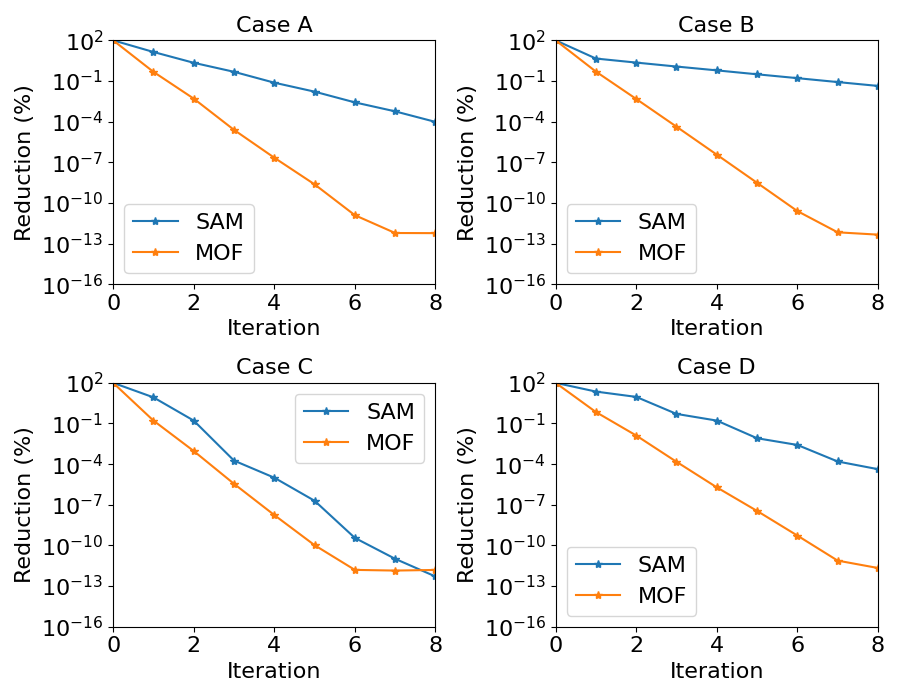
\includegraphics[angle=0,width=1.\textwidth]{fig/burgers-reduction_1.png}
  \caption{The residual reduction of Newton's method in different cases.}
  \label{fig:burgers-reduction}
\end{figure}
\subsubsection{Accuracy}
The accuracy study is conducted with two subdomains: $[-1, 0.25]$ and $[-0.25, 1]$. 
Both subdomains are meshed with uniform elements. In this investigation, 
we use $M^E_i=$ $25$, $50$, $100$, $200$, and $\Delta t=0.01$. \\
\begin{figure}[!htbp]
	\centering
	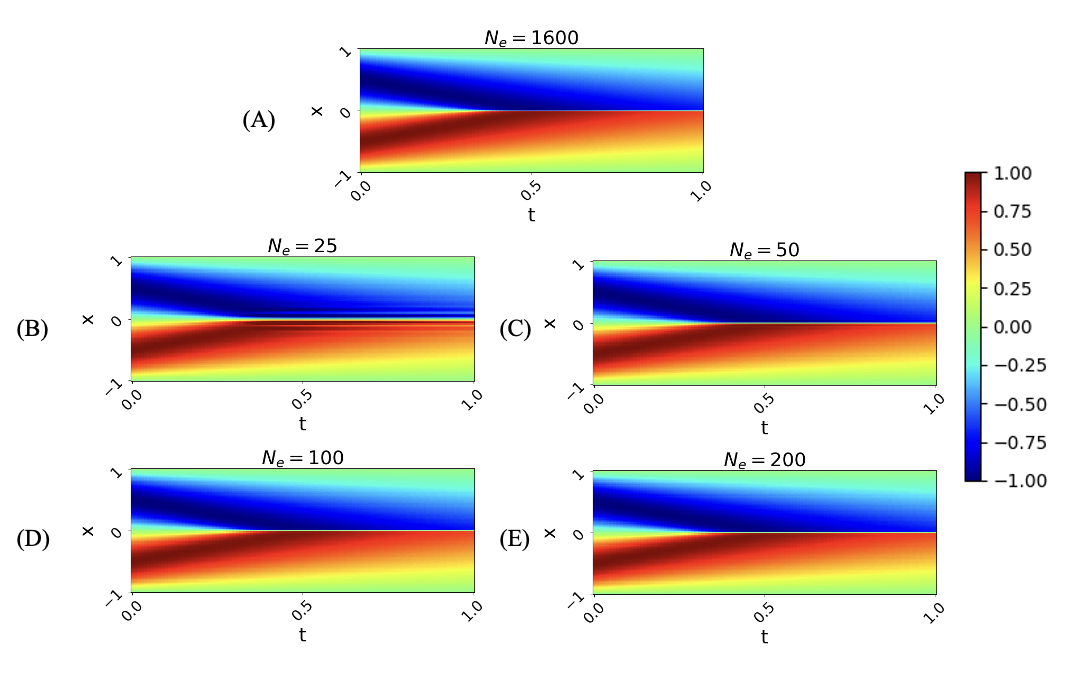
\includegraphics[angle=0,width=1.\textwidth]{fig/burgers-sol.png}
	\caption{The monolithic overset solution of Burgers' equation with $M^E_i=25,50,100,200$, compared with the single-mesh solution using $M_i^E=1600$.}
	\label{fig:burgers-fullfield}
\end{figure}
% Fig.~\ref{fig:burgers-fullfield} shows the solutions of Burgers' equation within $[-1, 1]\times[0,1]$ with $M_i^E=25,50,100,200$ using the monolithic overset method, compared with the single mesh solution $M_i^E=1600$.
Fig.~\ref{fig:burgers-fullfield} shows the solutions of the equation within $[-1, 1]\times[0,1]$ for $M^E_i=1600$ using the monolithic overset method and $M_i^E=25,50,100,200$ using the monolithic overset method.
The monolithic overset solutions agree with the single mesh solution when the mesh is sufficiently fine.
The difference between the single mesh solution and the monolithic overset solution in the overlapping region $[-0.25, 0.25]$ is defined as $\sqrt{ (|u_1-u_0|^2+|u_2-u_0|^2)/2}$ and plotted in Fig.~\ref{fig:burgers-diff}.
The discrepancy drops dramatically with the increase in mesh resolutions.
The difference mainly resides in the region close to the middle of the domain, where the solution meets the largest gradient.\\ 
\begin{figure}[!htbp]
	\centering
	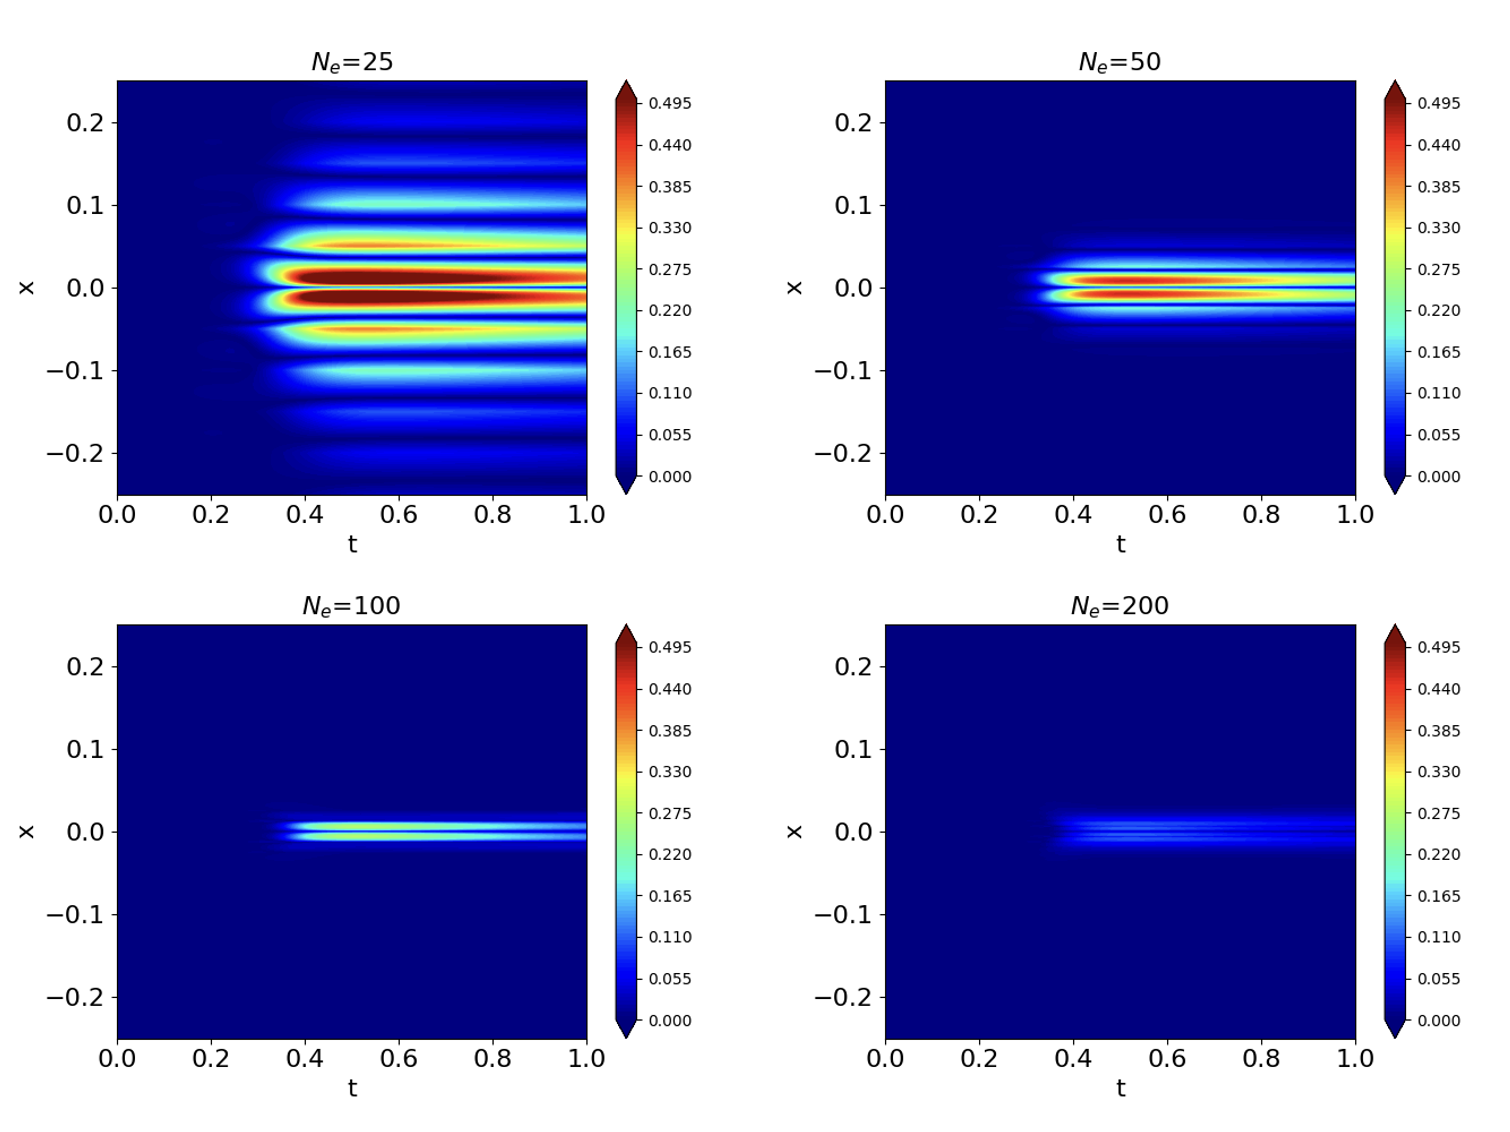
\includegraphics[angle=0,width=0.9\textwidth]{fig/burgers-diff.png}
	\caption{The difference between the single mesh solution $u_0$ ($M_i^E=1600$) and the monolithic overset solutions $u_1$ and $u_2$ ($M_i^E=25,50,100,200$) in the overlapping region [-0.25, 0.25]. The difference is defined as $\sqrt{ (|u_1-u_0|^2+|u_2-u_0|^2)/2}$. With the increasing mesh resolution, the discrepancy is dropping dramatically.}
	\label{fig:burgers-diff}
\end{figure}
The convergence of the monolithic overset method is plotted in Fig.~\ref{fig:burgers-convergence} in terms of $L_2$ error. The element length, $h=1.25/M_i^E$,
is used as the characteristic length. The convergence rate is close to 2, indicating the second-order accuracy of the proposed method, which is the optimal convergence rate of linear finite elements.\\
\begin{figure}[!htbp]
  \centering
	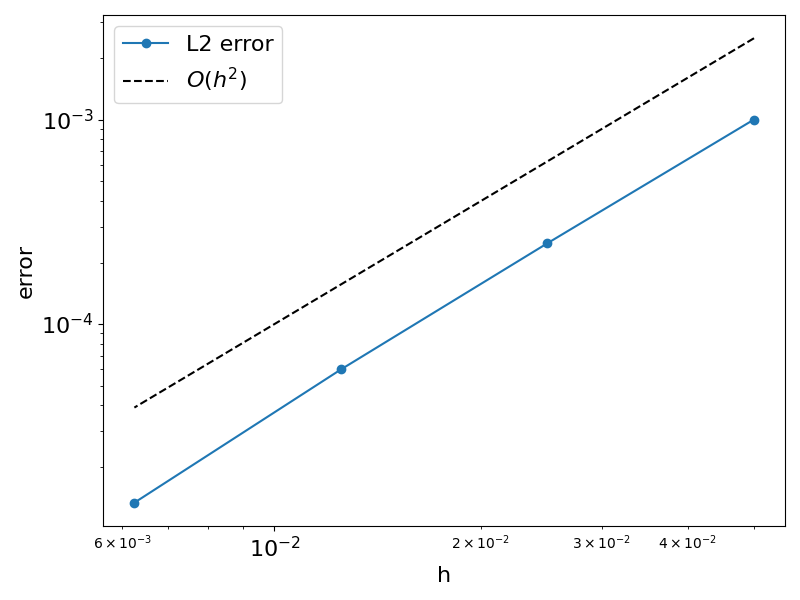
\includegraphics[angle=0,width=0.9\textwidth]{fig/burgers-convergence_1.png}
  \caption{The convergence of the monolithic overset method in Burgers' equation in terms of $L_2$ error.}
	\label{fig:burgers-convergence}
\end{figure}
This example demonstrates the feasibility of the proposed monolithic overset method in nonlinear FEM.
By comparing to a single-mesh approach, the proposed method yields good accuracy with a higher convergence rate and less computation time. Furthermore, the proposed method is validated through a more complicated engineering application, and the details are introduced in the following sections. 
%The results show that the proposed method is compatible with nonlinear FEM, and the accuracy is comparable with the single mesh solution. The following example further validates the proposed method with a more complicated scenario.

%\textcolor{red}{(Please ignore this paragraph) Fig.~\ref{fig:burgers} (A) depicts the contour of the solution field in the temporal-spatial domain $\Omega\times$[0,1]. Also, we plot the instantaneous solution comparison between the proposed method and the conventional single mesh method at time steps 0.25, 0.50, and 0.75 in Fig.~\ref{fig:burgers} (B-D). We obtain similar solutions at all time steps, indicating the accuracy of the monolithic framework in the overlapping meshes. In Fig.~\ref{fig:burgers} (E-F), we also present the absolute differences between two representations in overlapping regions. The solutions in the regions shared by two subdomains show remarkable agreements, and with increasing mesh resolutions, the error drops dramatically.}
\subsection{Hybrid Fliers}
% \textcolor{red}{AF: autorotating flier. PF: parachute flier. ALE: arbitraty Lagragian Eulerian. RMS: root mean square}
In creating lightweight, efficient, and environmentally harmonious flier systems for passive atmospheric exploration,
inspiration can be taken from seed dispersion phenomena in nature~\cite{kim2023flier,iyer2022wind}. Some plants have introduced sophisticated mechanisms to ensure 
the propagation of their species, with a subtle reliance on aerodynamics for their seeds to travel vast distances. Studying 
these natural systems can help us gain insights into inherently optimized aerodynamic designs. For example, parachuting dandelion 
seeds utilize separated vortex rings (SVRs) located above their center, and autorotating maple seeds utilize leading-edge vortices 
(LEVs) near their wing tip to generate lift and sustain flight~\cite{cummins2018separated, lentink2009leading}. Artificial flier systems aim to 
mimic these natural aerodynamic mechanisms and achieve a higher degree of stability and range by directly applying the evolutionary 
principles proven to work through millions of years. The study of the aerodynamic characteristics of these seeds enables informed 
design of passive flier systems that could revolutionize environmental monitoring and data collection, analogous to how nature has 
produced seed design for maximum dispersal efficiency.\\
% We set up the *flier system details, physical dimensions, * rotation parameters * AF and PF differences * spacing of the fliers * 
% We employ an Arbitrary Eulerian-Lagrangian approach on each of the \\
As shown in Fig.~\ref{fig:flier-seed}, the numerical study focuses on the interaction between the autorotating flier (AF) and 
parachute flier (PF), inspired by the dandelion and maple seeds, respectively. To mimic the geometry of the seeds, we use two CAD
models shown in Fig.~\ref{fig:flier-CAD}. Both models share the same diameter of $D=17.8\,\mathrm{mm}$.
In the setup, AF is placed in front of PF with a distance of $L=2D$ in a uniaxial way. The angular velocity of AF is 
$\omega=91.1\,\mathrm{rad/s}$ along the minus x-axis , and the incoming flow is $U_\infty=1.11\,\mathrm{m/s}$.
Moreover, the fluid density is $1$ $\mathrm{kg/m^3}$ and the density is $1.5\times 10^{-5}$ $\mathrm{Pa\cdot s}$.
The simulation is performed in a cylindrical domain of 0.16 $\mathrm{m}$ in diameter and 0.14 $m$ in length.
The domain is large enough to ensure the wall effect is negligible.
The time step is $\Delta t=5\times 10^{-5}$ $\mathrm{s}$, and the simulation lasts for 0.9 $\mathrm{s}$, sufficient for the system to reach a steady state.
Besides, the relative residual for Newton solver
is $10^{-3}$.\\
\begin{figure}[!htbp]
    \centering
    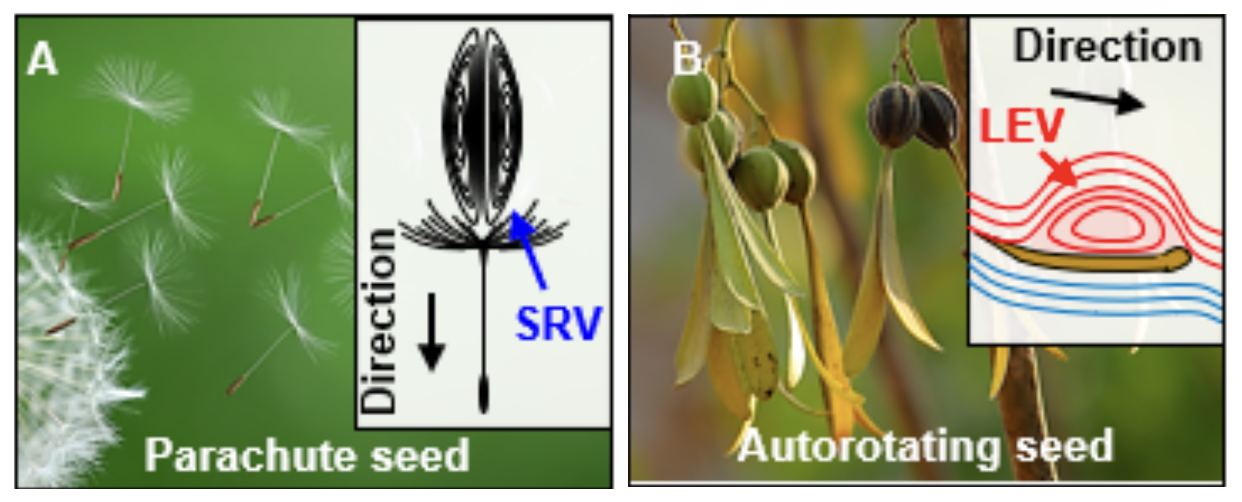
\includegraphics[angle=0,width=0.8\textwidth]{fig/flier-seed.png}
    \caption{The parachute and autorotating seeds in nature~\cite{kim2023flier}.}
    \label{fig:flier-seed}
\end{figure}
\begin{figure}[!htbp]
    \centering
    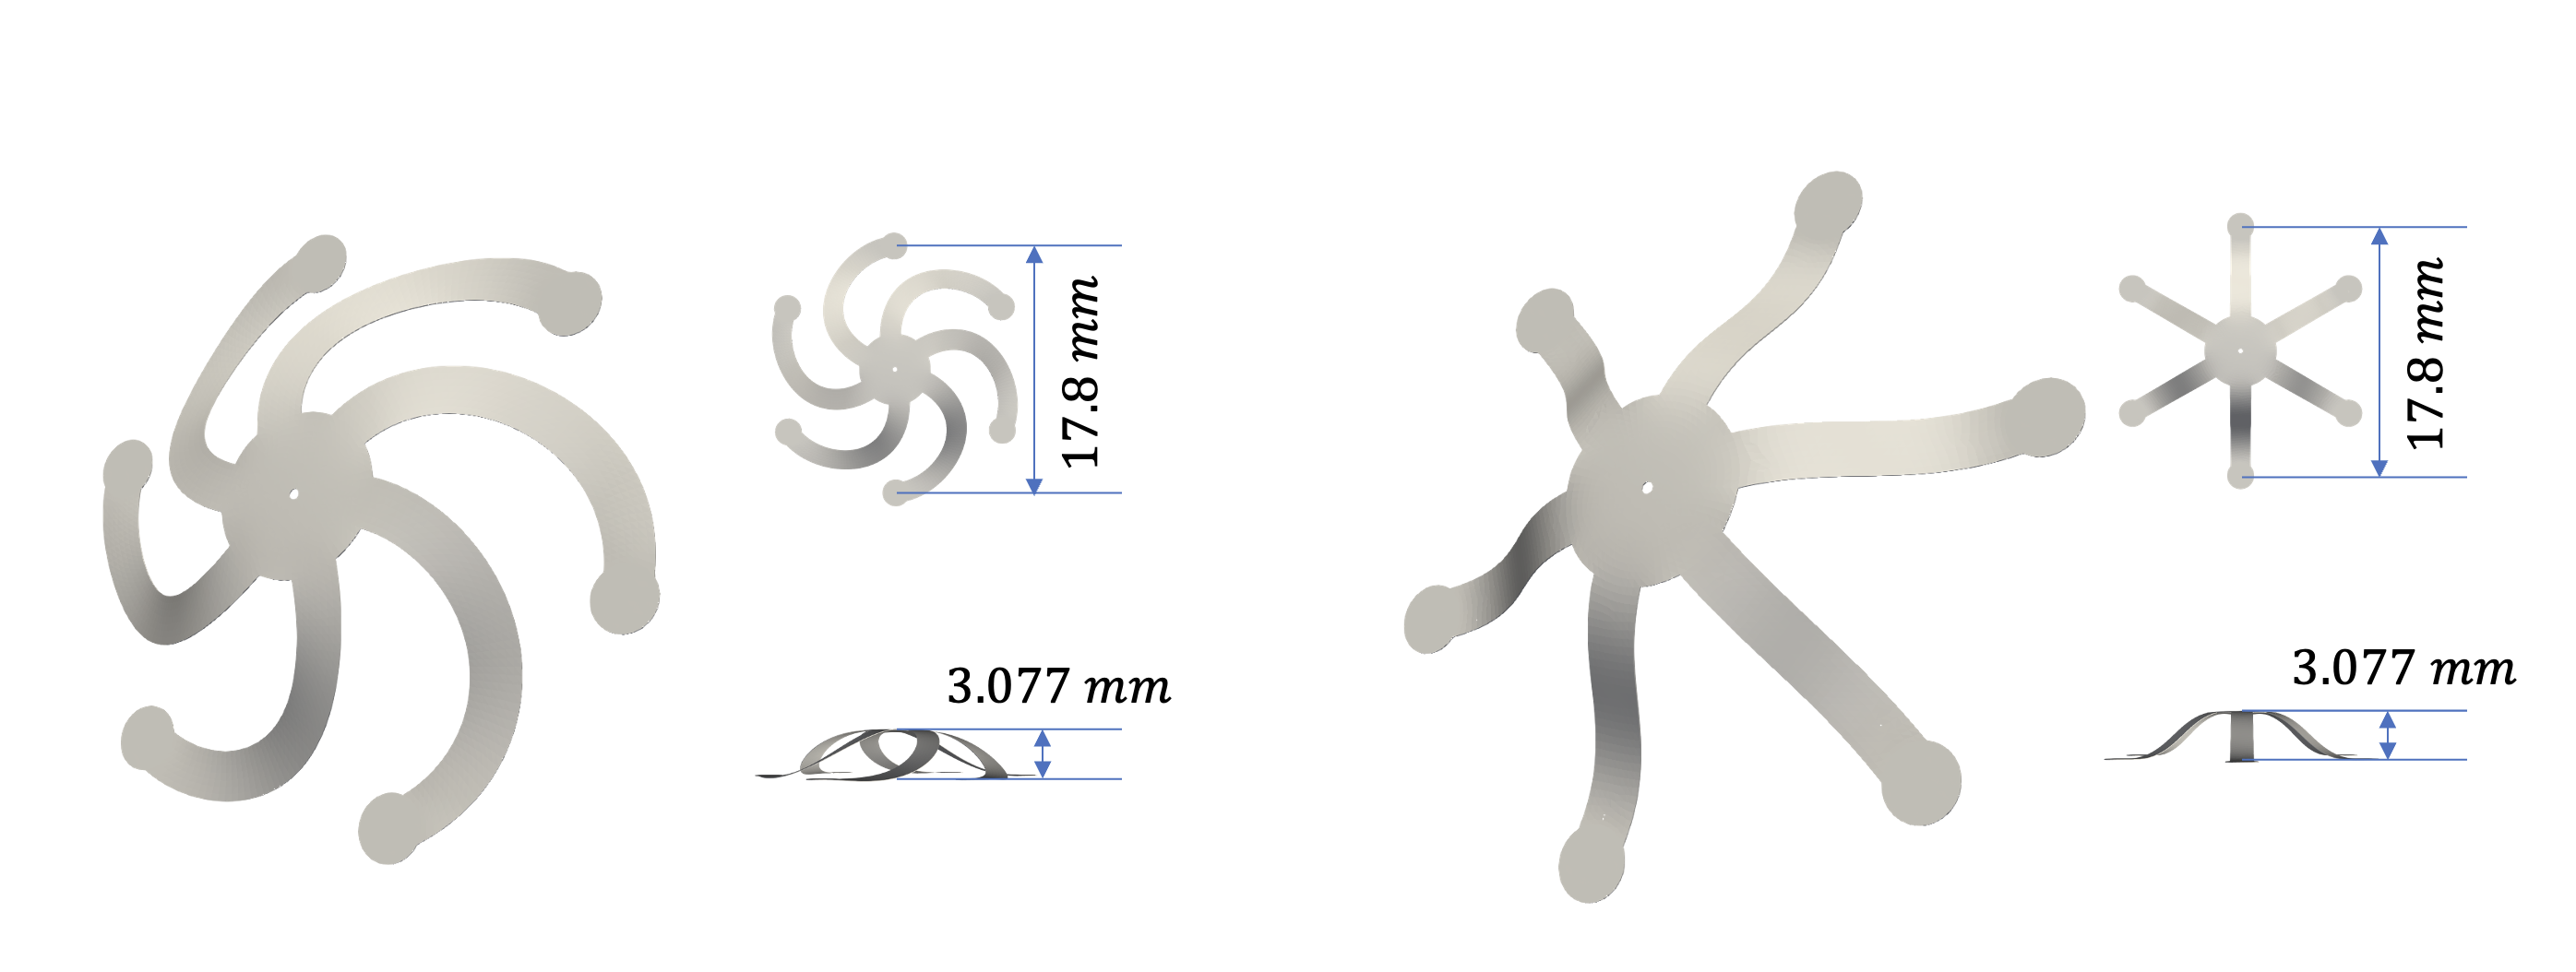
\includegraphics[angle=0,width=0.9\textwidth]{fig/flier-CAD.png}
    \caption{The CAD model and dimensions of AF and PF.}
    \label{fig:flier-CAD}
\end{figure}
We generate the mesh as shown in Fig.~\ref{fig:flier-mesh}, which includes two independent meshes for AF and PF. 
The mesh resolution is as fine as $5\times 10^{-4}\,\mathrm{m}$, and the 
mesh contains 6,485,933 tetrahedrons and 1,142,545 nodes in total.
The mesh is designed to maintain an overlapping region between two disconnected parts, as shown by two cylinders. 
As discussed in Section~\ref{sec:monolithic-overset-framework}, the surfaces where the solution continuity is 
enforced act as both the external boundaries of one mesh and the internal boundaries of the other mesh.
The overlapping size is crucial for the convergence of the overset method and
we keep the overlapping region containing up to 10 layers of elements, which is a safe choice for the convergence.
The inner part of the mesh rotates with the flier using ALE, and the outer one stays stationary during the simulation.\\
\begin{figure}[!htbp]
    \centering
    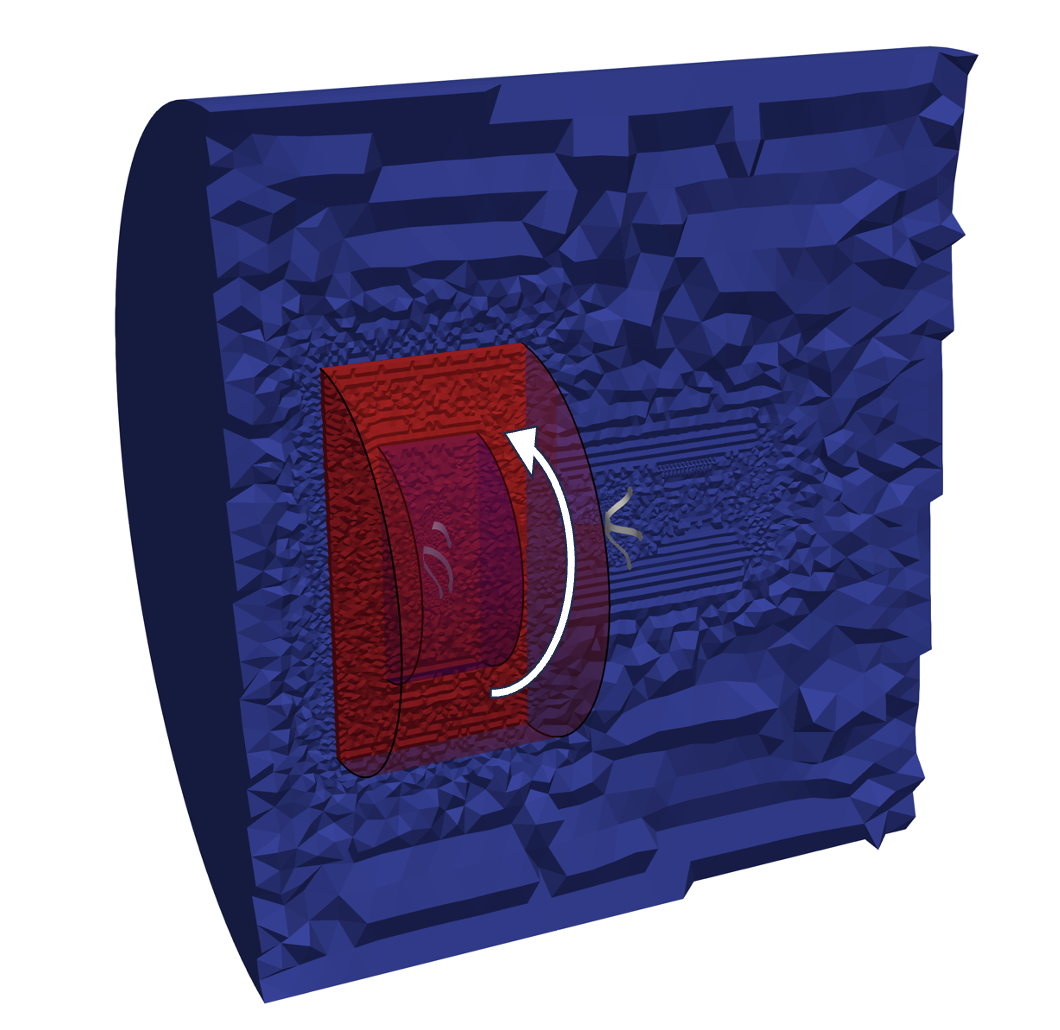
\includegraphics[angle=0,width=0.8\textwidth]{fig/flier-mesh.png}
    \caption{The mesh consists of 6,485,933 tetrahedrons and 1,142,545 nodes.}
    \label{fig:flier-mesh}
\end{figure}
\begin{figure}[!htbp]
    \centering
    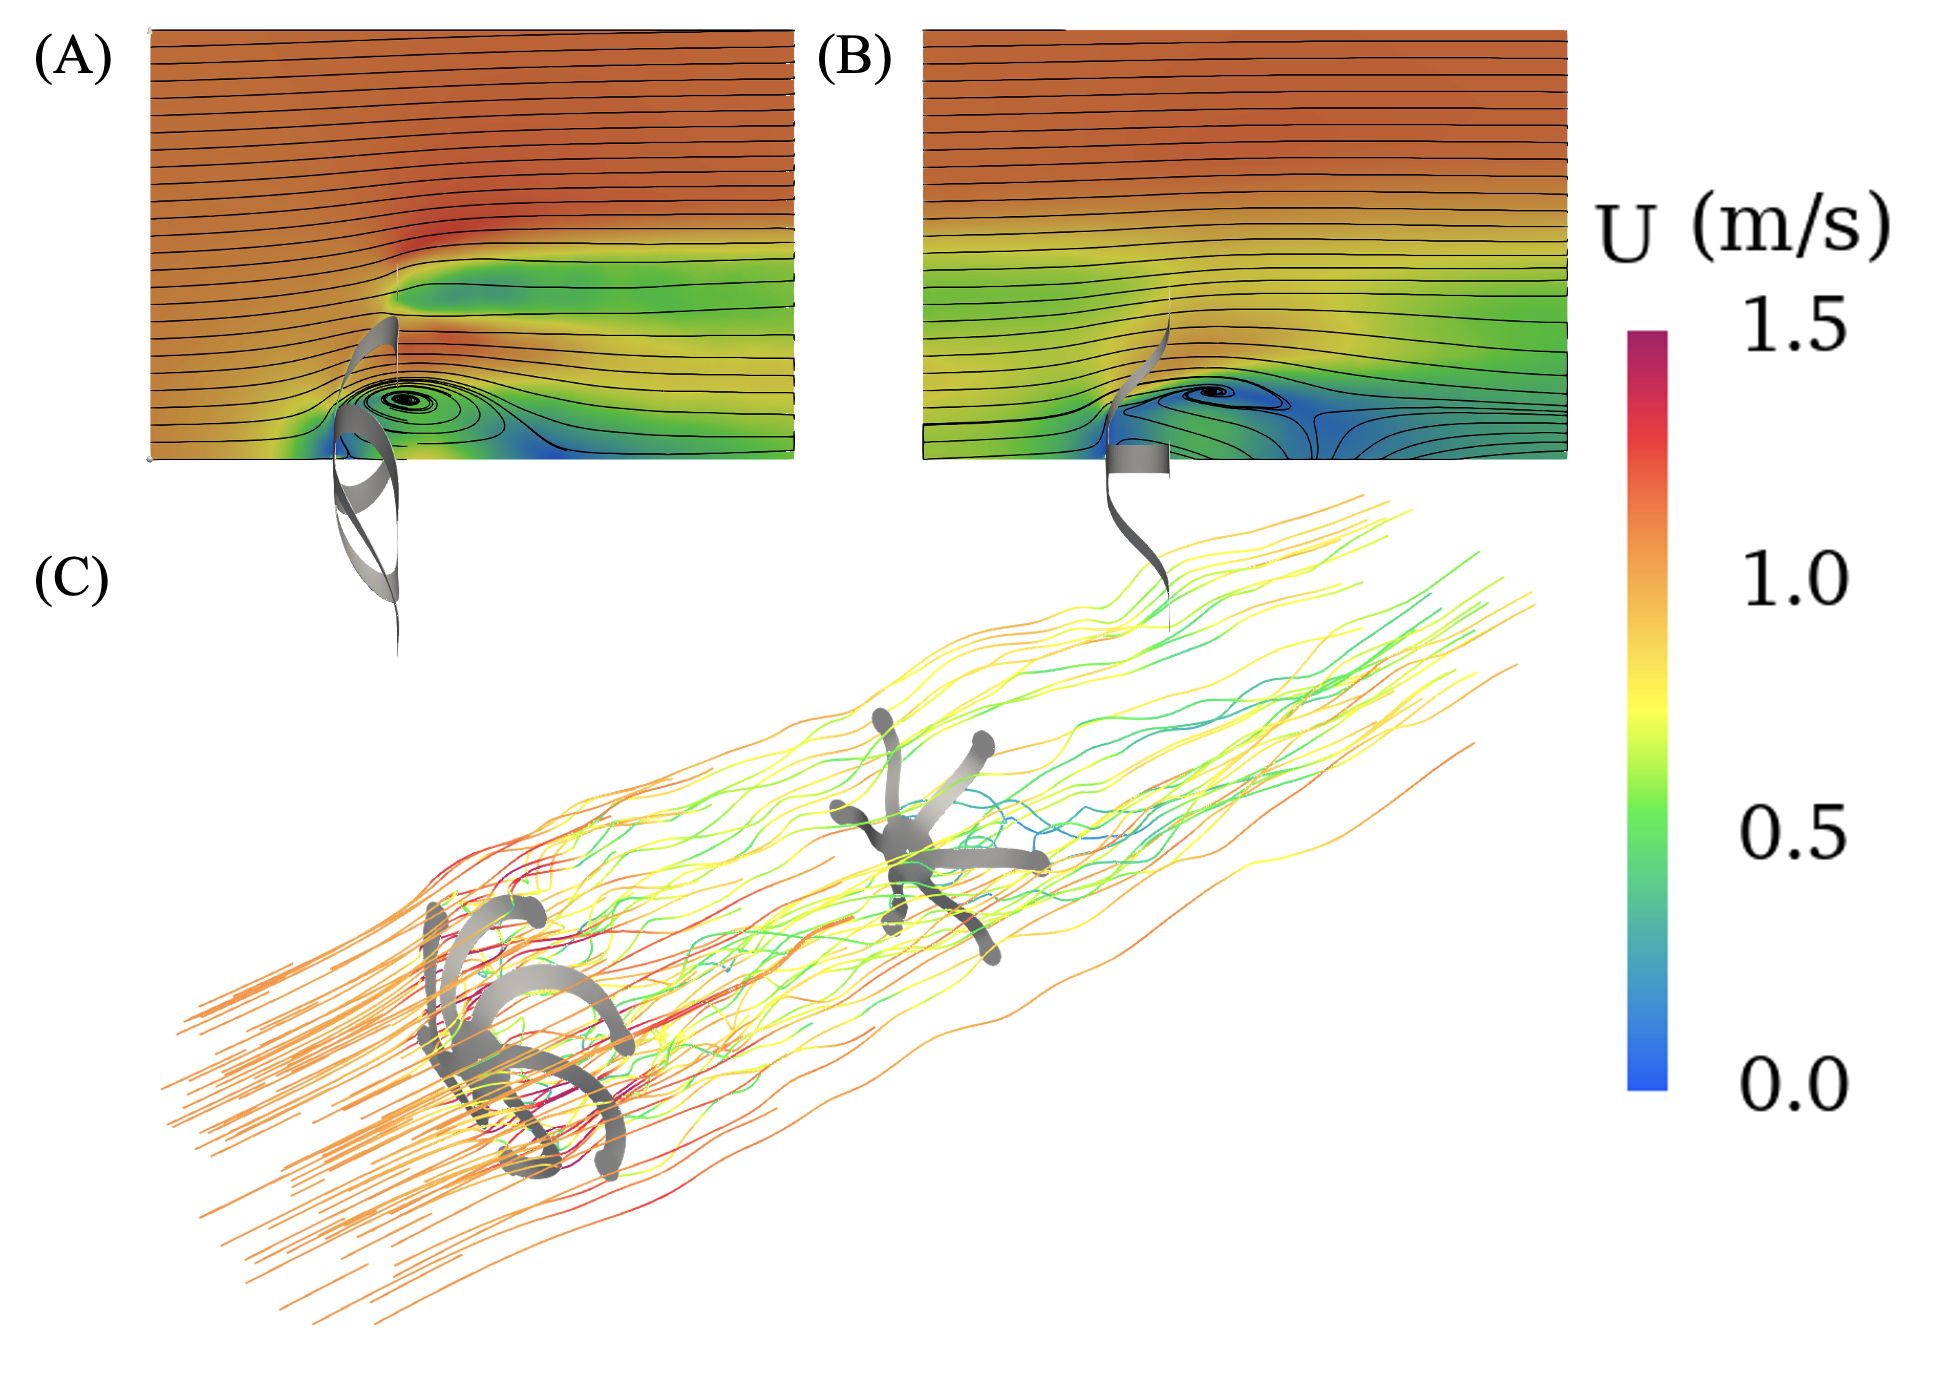
\includegraphics[angle=0,width=1.0\textwidth]{fig/flier-streamlines.png}
    \caption{The instantaneous and time-average streamlines around two fliers. (A) and (B) shows the time-averaged 
    streamline behind AF and PF. The flow forms circulations behind both structures. (C) presents the instantaneous 
    streamline through two fliers at $t$=0.25 $\mathrm{s}$.}
    \label{fig:flier-streamline}
\end{figure}
Fig.~\ref{fig:flier-streamline} depicts the instantaneous and time-average streamlines around two fliers. 
Fig.~\ref{fig:flier-streamline} (A) and (B) show the time average streamlines in the downstream of AF and PF, respectively.
AF and PF generate circulations behind them, indicating significant flow separation behind the structure. 
The induced drag strongly supports the flier from dropping to the ground and ensures it can travel as far as
possible. Fig.~\ref{fig:flier-streamline} (C) presents the instantaneous streamlines through two fliers at $t$=0.25 $\mathrm{s}$.
The flow is highly turbulent and complicated. The velocity field is disturbed by the flyer motion.
It is noticeable that the flow velocity decreases significantly after passing through AF, and the flow is almost stagnant behind PF.\\
\begin{figure}[!htbp]
    \centering
    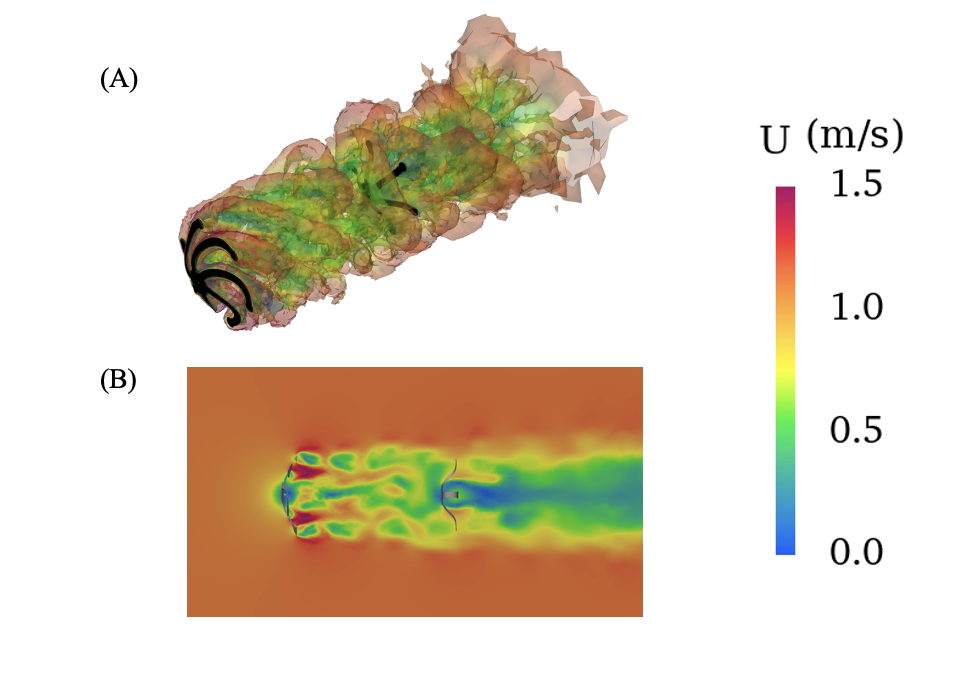
\includegraphics[angle=0,width=1.0\textwidth]{fig/flier-vorticity-velocity.png}
    \caption{The vorticity structure and the velocity magnitude. (A) shows the isosurface of the Q-criterion. (B) is the velocity magnitude on the center plane cut.}
    \label{fig:flier-qiso}
\end{figure}
Fig.~\ref{fig:flier-qiso} presents the turbulence structure and the velocity magnitude on the center plane cut. We use 
the isosurface of Q-criterion to identify the vortex structures, which is defined as
\begin{align}
  Q=\frac{1}{2}\bigg\vert\nabla\bm{u}:\nabla\bm{u}-\nabla\bm{u}:(\nabla\bm{u})^T\bigg\vert
\end{align}
Velocity magnitude is plotted on the center plane cut. Fig.~\ref{fig:flier-drag} validates our method in terms of the accuracy of 
the drag coefficient. The drag coefficient is defined using
\begin{align}
C_D=\frac{8F_D}{\pi \rho U_\infty^2 D^2}
\end{align}
where $F_D$ is the force along the streamwise direction. The drag coefficient history reaches a steady state rapidly after $t$=0.1 $\mathrm{s}$, and the numerical predictions agree
with the experimental data~\cite{kim2023flier}. We also conduct an ALE simulation of each single flier. The drag coefficient of the single AF simulation is the 
same as the other two. However, PF, behind AF in the simulation, has a lower drag coefficient than the single PF simulation. The difference
comes from the interaction between AF and PF. The turbulent flow generated by flow passing AF causes a remarkable drag decrease, which is not 
considered in the single flier simulation. The inevitable role of interaction between fliers demonstrates the necessity of the monolithic 
overset method.
\begin{figure}[!htbp]
    \centering
    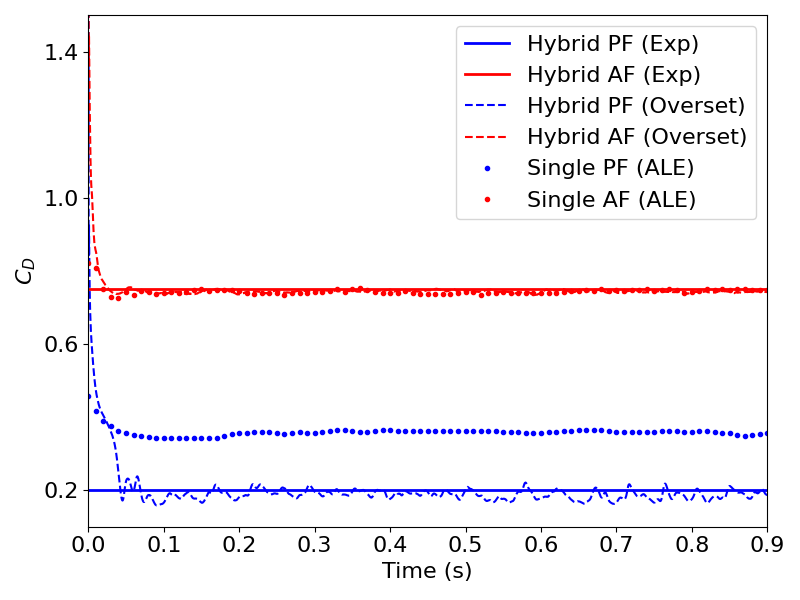
\includegraphics[angle=0,width=1.0\textwidth]{fig/flier-drag-coef_1.png}
    \caption{The drag coefficient of AF and PF.}
    \label{fig:flier-drag}
\end{figure}
We use the time interval of the last 0.2 $\mathrm{s}$ out of 0.9 $\mathrm{s}$ to calculate the time average. The mean velocity 
and root mean square (RMS) are shown within 0.03 $\mathrm{m}$ from the fliers. Due to the holes in the center of 
the CAD model, the mean velocity there is non-zero for AF and PF. Additionally, the rotating flier forms a strong blockage effect, significantly decreasing the minimal
mean velocity. The rotation is also attributed to the higher RMS because it introduces a strong vortex shedding.\\
\begin{figure}[!htbp]
    \centering
    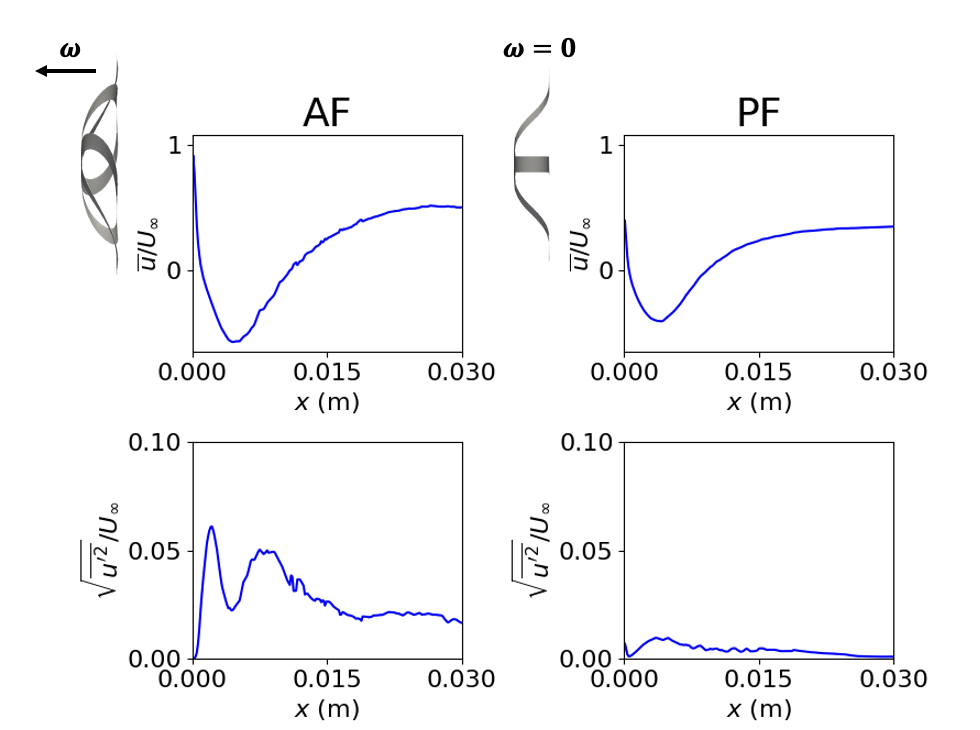
\includegraphics[angle=0,width=1.0\textwidth]{fig/flier-centerline-umean_3.png}
    \caption{The time-average and RMS of streamwise velocity generated using the data within $0.7 \mathrm{s} < t < 0.9 \mathrm{s}$.}
    \label{fig:flier-umean}
\end{figure}

\section{Conclusion}\label{sec:conclusion}
The proposed monolithic overset method addresses the limitations of the classic SAM, a popular solving technique for the overset
meshes. SAM shows low robustness and slow convergence as a domain decomposition method, eventually leading to inefficiency in
large-scale simulations.\\
The proposed method does not rely on the inter-mesh iteration and solves the overset system monolithically. By inserting the difference between
current values and the enforced Dirichlet boundary conditions into the residual, additional constraints for the solution continuity
are imposed on the alternating boundaries, which, in contrast, are treated as external boundaries in the classic SAM. The new constraints
make it feasible to evaluate the Jacobian matrix of the overset system. The general forms of the residual vector and Jacobian matrix 
are derived. Although the paper focuses on the incompressible Navier-Stokes equation,  the general form is compatible with many other problems.\\
We also investigate parallelization and collision detection as a part of the proposed method. Since the alternating residual is not derived from the weak form, the 
traditional assembly way is not applicable for both the residual and Jacobian matrix. Since GMRES, an iterative solver, is used
in each Newton iteration, Jacobian matrices are only used for preconditioning and matrix-vector multiplication. Therefore, we utilize a
composited and partially matrix-free Jacobian layout. Specifically, the submatrices derived from the weak form follow the conventional
assembly way, and the submatrices derived from the alternating residual are calculated by the matrix-free method, which includes interpolation
and subtraction serially. The layout is compatible with the parallelization of the Newton solver, and the efficiency is also remarkable,
given that the nodes of the alternative surfaces take up just a small portion of the whole mesh. An octree-based searching algorithm performs the collision detection required by interpolation. Both the construction and searching are highly efficient.\\
We apply the general form to two numerical examples. In Burgers' equation, we demonstrate the convergence by comparing the nonlinear 
residual reduction in Newton iterations with different mesh resolutions, time step lengths, and overlapping ratios. The residual of the monolithic overset method outperforms the single-mesh method in all test cases. The accuracy of the monolithic overset method is evaluated against the single-mesh solution with sufficient high resolutions.
Similar solutions are obtained in the overlapping region and all over the computational regions. The optimal convergence
rate for linear elements is observed for $h$-refinement. In the simulation of hybrid fliers, we validate the method with a pair
of uniaxial fliers. The inconsistent rotational speeds and high requirement for drag prediction provide an ideal test case for the 
monolithic overset method, where neither boundary-fitted ALE nor immersed boundary method is suitable. The visualization of the circulations
shows the flow separation behind the fliers, consistent with the time-averaged mean velocity profile. We also plot the drag coefficients
of two fliers, collapsing with the experimental data. The drag coefficient of the single flier simulation is also plotted. The upstream flier
is similar, but the downstream one is significantly different, indicating that the turbulence generated by the first flier is imminent to capture
the drag of filers in the wakes. The importance of flier interaction provides strong support for the monolithic overset method. The numerical
examples illustrate that the goals of the method are well satisfied.

\section*{Acknowledgment}\label{Ack}
J. Yan was partially supported by the U.S. Department of Energy under the grant of DE-EE0009447. The support is greatly acknowledged.
\newpage
\bibliographystyle{unsrtnat}
%\bibliographystyle{plain}
\bibliography{ref}
%\end{multicols}

\end{document}
